\documentclass[7pt,landscape, margin = 0.1mm]{article}
\usepackage{amssymb,amsmath,amsthm,amsfonts}
\usepackage{multicol,multirow}
\usepackage{graphicx}
\usepackage{float}
\usepackage{calc}
\usepackage[dvipsnames]{xcolor}
\usepackage{ifthen}
\usepackage{titlesec}
\usepackage[landscape]{geometry}
\usepackage{enumitem}
\usepackage{syntonly}
\setitemize{noitemsep,topsep=0pt,parsep=0pt,partopsep=0pt}
\usepackage[colorlinks=true,citecolor=blue,linkcolor=blue]{hyperref}
\usepackage{tikz}
\def\cm{\tikz\fill[scale=0.4](0,.35) -- (.25,0) -- (1,.7) -- (.25,.15) -- cycle;} 
\ifthenelse{\lengthtest { \paperwidth = 11in}}
    { \geometry{top=.1in,left=.1in,right=.1in,bottom=.1in} }
	{\ifthenelse{ \lengthtest{ \paperwidth = 297mm}}
		{\geometry{top=1mm,left=1mm,right=1mm,bottom=1mm} }
		{\geometry{top=1mm,left=1mm,right=1mm,bottom=1mm} }
	}

\pagestyle{empty}

\makeatletter

 

\newcommand{\nextcol}{\vfill\null\columnbreak}

\newcommand{\titellinie}{\rule{1.\linewidth}{0.75pt}}

\titleformat{\subsection}
  {\normalfont\fontsize{10}{10}\bfseries}{\thesection}{1em}{}

\newcommand*{\mysection}[2][black]{\vskip 0pt \titellinie\vspace{-20pt}\section{#2}\vspace{-14pt}\titellinie \colorlet{chaptercolor}{#1}}

\newcommand*{\mysubsection}[1]{\vspace{-2mm}\color{chaptercolor}\subsection{ #1 }
\vspace{-1mm}\hrule\vspace{1.5mm}\color{black}
\vspace{2mm}}

\newcommand{\COL}[1]{ \color{chaptercolor} \bf{#1}\color{black}     \\}


\newcommand{\KRZ}[2]{\vspace{1mm} \hline \vspace{1mm} \color{chaptercolor}{RC #1}:\color{black} \   \hspace{0.2cm}\vspace{1mm}   {\begin{minipage}{20em}
#2 \end{minipage}} \vspace{1mm}  \hline \vspace{1mm}  \\}


\newcommand{\DEF}[2]{\color{chaptercolor}\bf{Def #1}:\color{black}    \hspace{0.2cm} #2 \\}

\newcommand{\NOTE}[2]{\color{chaptercolor}\bf{Note #1}:\color{black}    \hspace{0.2cm} #2 \\}

\newcommand{\COR}[2]{\color{chaptercolor}\bf{Cor #1}:\color{black}    \hspace{0.2cm} #2 \\}

\newcommand{\LEM}[2]{\color{chaptercolor}\bf{Lem #1}:\color{black}    \hspace{0.2cm} #2 \\}

\newcommand{\THE}[2]{\color{chaptercolor}\bf{Trm #1}:\color{black}    \hspace{0.2cm} #2 \\}
\newcommand{\SA}[2]{\color{chaptercolor}\bf{S #1}:\color{black}    \hspace{0.2cm} #2 \\}

\makeatother
\setcounter{secnumdepth}{0}
\setlength{\parindent}{0pt}
\setlength{\parskip}{0pt plus 0.5ex}
\setlength{\marginparwidth}{0pt}
\setlength{\marginparsep}{0pt}
% -----------------------------------------------------------------------
\begin{document}
\syntaxonly
\centering

\scriptsize

\begin{center}
     \Large{\textbf{Cheat Sheet}: Comp Sc BSc, LinAlg - Brian Funk, 21.04.2001 - \textbf{22-918-18-957}} \\
\end{center}
\begin{multicols}{4}
\setlength{\premulticols}{0.5pt}
\setlength{\postmulticols}{0.5pt}
\setlength{\multicolsep}{0.5pt}
\setlength{\columnsep}{0.2pt}
\setlength{\columnseprule}{0.4pt}

\begin{flushleft}

\mysection[BrickRed]{\centering Complex Numbers}
\mysubsection{\centering Basics}
\DEF{}{$z = a + bi \Leftrightarrow \Re (z)=a, Im(z)=b $}
\DEF{}{$z = a + bi \Leftrightarrow \bar{z} = a - bi \Leftrightarrow r \cdot e^{2\pi- \phi}$}
\DEF{}{$z = r \cdot cos(\phi)+ i\cdot sin(\phi) $}
\DEF{}{$|z| = r = \sqrt{x^2 + y^2} = \sqrt{z \cdot \bar{z}} $}
\DEF{}{$ \phi = \begin{cases}
arctan \frac{y}{x} & \text{1. Q} \\
arctan \frac{y}{x} + \pi & \text{2./3. Q}  \\
arctan \frac{y}{x} + 2pi& \text{4. Q}  
\end{cases} $}
\mysubsection{\centering Operations}
\DEF{}{$ z_1\pm z_2: (x_1 + x_2) \pm i(y_1 + y_2) $}
\DEF{}{$ z_1\cdot z_2: (x_1 + i \cdot y_1)+ (x_2 + i \cdot y_2) = r_1 \cdot r_2 e^{i(\phi_1 + \phi_2)}$}
\DEF{}{$ \frac{z_1}{z_2}:\frac{r_1}{r_2}e^{i(\phi_1 - \phi_2)} = \frac{z_1 \cdot \bar{z_2}}{|z_2|^2}$}
\DEF{}{$ \sqrt[n]{a} \Leftrightarrow a = z^n \Leftrightarrow |a|\cdot e^{i \phi}= r^n \cdot e^{i \omega n} \Leftrightarrow r = \sqrt[n]{|a|}, \omega = \frac{\phi + 2k\pi}{n}$}
\mysubsection{\centering Polynomials}
The roots of a complex polynomial are pairwise conjugated.
\DEF{}{$z = \frac{b \pm \sqrt{b^2 -4ac}}{2a}$}
\DEF{}{$ az^n + c= 0  \Leftrightarrow z= \sqrt[n]{-\frac{c}{a}}  $}
\begin{Figure}
 \centering
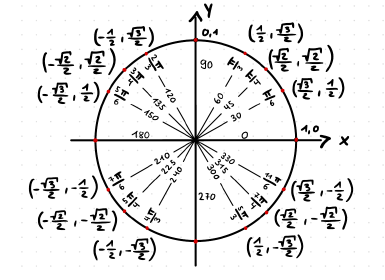
\includegraphics[width=\linewidth]{pictures/complex numbers.png}
\end{Figure}


\mysection[BurntOrange]{\centering SLE}
\mysubsection{\centering Gauss Algorithm}

\begin{Figure}
 \centering
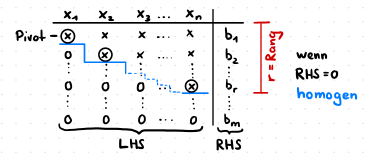
\includegraphics[scale=1]{pictures/Gauss.png} 
\end{Figure}
\color{chaptercolor} Compability Conditions: \color{black} $b_{r+1}=...=bm=0 $\\
\SA{1.1}{$Ax = b $ hat min eine Lösung $\Leftrightarrow r = m $ oder $ r<m + \color{chaptercolor} VB \color{black}$ dann:  $ r=n \Leftrightarrow  1 $ Lösung , $ r<n \Leftrightarrow \infty $ Lösungen } \\
\COR{1.7}{For a quadratic SLE with $n$ equations and $n$ variables we have the following set of equivalence, of wich ONLY one of them can be true; So, EITHER
\begin{itemize}
\item[i] $Rank(A) = n$ (A is regular)
\item[ii] for every $b$ there exist at least one solution
\item[iii] for every $b$ there exists exactly one solution
\item[iv] the corresponding homogeneous system has only the trivial solution 
\end{itemize}
\\ OR the following equivalences hold \\
\begin{itemize}
\item[v] $Rank(A) < n$ (A is singular)
\item[vi] for some $b$ there exits no solution
\item[vii] for no $b$ a unique solution exists
\item[viii] for some $b$ infinity many solution exists
\item[ix] the corresponding homogeneous system has non-trivial solutions
\end{itemize}
}
\\
\mysection[Dandelion]{\centering Matrices and Vectors}
\mysubsection{\centering Definitions}
A $m \times n  $ matrix hat m \COL{row (Zeilen)$\downarrow$}  and n \COL{columns (Spalten)$\to$}, in which the i,j element gets noted by $a_{i,j}$ or $(A)_{i,j} $\\
\DEF{nullmatrix}{Has in every entry $0$}
\DEF{diagonalmatrix}{Has in every entry $0$ except for the diagonal: $(D)_{ij} = 0$ for $i \neq j $ one can write $Diag(d_{11}, \cdots , d_{nn}) $}
\DEF{identity}{The identity is written as $I_n = Diag(1 , \cdots , 1)$ It holds that $AI = IA = A $}
\DEF{upper triangular matrix}{We have $(R)_{ij} = 0$ for $i > j $ (Rechtsdreiecksmatrix)}
\DEF{lower triangular matrix}{We have $(R)_{ij} = 0$ for $i < j $ (Linksdreiecksmatrix)}
\DEF{Matrix-set}{The set of $ m \times n $-matrices is written as: $\mathbb{E}^{m \times n } $ For vectors we have: $ \mathbb{E}^{n}$, where $ \mathbb{E}$ is $ \mathbb{R}$ or $ \mathbb{C}$ }
\DEF{matrix multiplication}{If $C =AB $ then one can write $C_{ij} = (AB)_{ij} = \sum_{k=1}^{n} (A)_{ik}(B)_{kj} = \sum_{k=1}^{n} a_{ik}b_{kj}   $}
\SA{2.1}{\begin{itemize}
\item $(\alpha \beta)A= \alpha (\beta A)$
 \item $(A+B)+C= A+(B+C)$
 \item  $(\alpha A)B= \alpha (AB)$ 
 \item $(AB)\cdot C = A \cdot(BC)$
 \item $(\alpha + \beta)A= \alpha A + \beta A $
 \item $(A+B)\cdot C = AC+BC $
 \item $ A\cdot (B+C) = AB+AC $
 \item $ \alpha (A+B)= \alpha A + \alpha B$
 \item $A+B=B+A$
 
\end{itemize}}
\SA{2.20}{Let $A $ and $B$ be unitary(orthogonal). It holds:
\begin{itemize}
\item $A$ is regular and $A^{-1}=A^H (A^T) $
\item $AA^H (AA^T) = I $
\item $A^{-1} $ is unitary (orthogonal)
\item  $AB $ is unitary (orthogonal)
\end{itemize}

}
\DEF{Zerodiviser}{If $AB=0  \Leftrightarrow $ A,B Zerodiviser, Nullteiler}
\DEF{transposes}{ $ (A^T)_{ij}=A_{ji} $}
\DEF{conjugate transposed}{$ A^H = (\overline{A})^T=\overline{A^{T}}$}
\DEF{symmetric}{$A^T = A  \Leftrightarrow $A symmetric}
\DEF{skew-symmetric}{$A^T = -A  \Leftrightarrow $A skew-symmetric}
\DEF{hermitian}{$A^H = A  \Leftrightarrow $A hermitian}
\SA{2.6}{  Also accounts for $A^T $ instead of $A^H$.
$ \overline{ \alpha} $ simplifies to $\alpha $ 



\begin{itemize}
\item $(A^H)^H=A $
\item $(\alpha A)^H=\overline{\alpha} A^H $
\item $(A+B)^H=A^H+B^H$
\item $ (AB)^H=B^H A^H$
 
\end{itemize}}
\SA{2.7}{For symmetric matrices $A$ and $B$ it holds that: 
$AB=BA \Leftrightarrow AB $ is symmetric
It holds for arbitrary matrix $C$ that:
$C^T C$ and $ CC^T$ are symmetric. The same holds for the hermitian case}
\mysubsection{\centering Scalarproduct and Norm}
\DEF{euclidian scalarproduct}{ $\left< x,y\right> = x^T y = \sum_{k=1}^{n} \overline{x_k} \cdot y_k \xrightarrow[ \mathbb{R}]{in}\sum_{k=1}^{n} x_k \cdot y_k$}
\SA{2.9}{\begin{itemize}

\item[S1] $ \left< x,y+z\right>=\left< x,y\right>+\left< x,z\right> $(linear in 2nd factor)
\item[S1] $ \left< x,\alpha y\right> = \alpha\left< x,y\right>$ (linear in 2nd factor)
\item[S2] for $ \mathbb{E} = \mathbb{R}$:\\$\left< x,y\right>=\left< y,x\right>$ (symmetric)
\item[S2'] for $ \mathbb{E} = \mathbb{C}$:\\$ \left< x,y\right>=\overline{\left< y,x\right>}$(hermitian)
\item[S3] $ \left< x,x\right> > 0, \left< x,x\right>=0\Leftrightarrow x=0$(positiv definite)
 
\end{itemize}}
\COR{2.10}{\begin{itemize}
\item[S4] for $\mathbb{E} = \mathbb{R} $: linear in 1st factor
\begin{itemize}
\item[] $ \left< w+x,y\right>=\left< w,y\right>+\left< x,y\right> $
\item[]  $ \left<\alpha x , y\right> = \alpha\left< x,y\right> $
\end{itemize}
\item[S4'] for $\mathbb{E} = \mathbb{C} $: conjugate-linear in 1st factor 
\begin{itemize}
\item[] $ \left< w+x,y\right>=\left< w,y\right>+\left< x,y\right> $
\item[] $ \left< \alpha x , y\right> = \overline{\alpha}\left< x,y\right> $
\end{itemize}
\end{itemize}}



\DEF{norm}{$ \left\|x \right\| = \sqrt{\left< x,x\right>}=\sqrt{x^T x} = \sqrt{\sum_{k=1}^{n} (|x_k|)^2} \xrightarrow[\mathbb{R}]{in} \sqrt{\sum_{k=1}^{n} x_k^2}$}
\SA{2.11}{$|\left< x,y\right>| \leq \left\|x \right\| \cdot  \left\|y \right\|$( Cauchy-Schwarz inequality, "=" holds when y is a multiple of x or vice verca)}
\DEF{CBS}{CBS is a property of the scalar product: CBS squared yields: $|\left< x,y \right>|^2 \leq \left< x,x \right>\left< y,y\right> $}
\SA{2.12}{For the euclidian norm holds: \begin{itemize}

\item[N1] $ \left\|x \right\| > 0 , \left\|x \right\| = 0 \Leftrightarrow x=0$(positiv definit)
\item[N2] $\left\|\alpha x \right\| = \alpha \left\|x \right\| $ (homogeneous)
\item[N3] $\left\|x \pm y \right\| \leq \left\|x \right\| + \left\|y \right\|$ (Triangle-inequality)
\end{itemize}} 
\DEF{}{Angle $\phi$ between $x,y$: $ ,\phi = arccos \frac{Re (\left< x,y\right>)}{ \left\|x \right\| \cdot \left\|y \right\|}\xrightarrow[\mathbb{R}]{in} arccos \frac{\left< x,y\right>}{ \left\|x \right\| \cdot \left\|y \right\|}$}
\DEF{}{$x,y$ are orthogonal: $\left< x,y\right>=0 \Leftrightarrow x \perp  y $}
\SA{2.13}{$\left\|x \pm y \right\|^2 = \left\|x \right\|^2 + \left\|y \right\|^2 \Leftrightarrow x \perp  y$}(Pythagoras)
\DEF{p-norm}{$\left\|x\right\|_p = \left ( \left| x_1 \right|^p \cdots \left| x_n \right|^p \right )^{\frac{1}{p}$}}


\mysubsection{\centering Outer Product and Projections}
\DEF{outer product}{m-vector $x$ and n-vector $y$: $xy^T$}
\SA{2.14}{A $m \times n $-matrix has rank 1 if it is the outer product of an m-vector $\neq 0 $ and n-vector $\neq 0 $}
\SA{2.15}{ The orthogonal projection $P_yx $ of the n-vector $x$ onto y is defined as: $P_yx=\frac{1}{\left\|y \right\|^2}\cdot yy^Hx = uu^H= P_u$ where $u = \frac{y}{\left\|y \right\|} $}
\DEF{projections matrix}{$P_y=\frac{1}{\left\|y \right\|^2}\cdot yy^H$ It has the properties: $P_y^H=P_y $ (hermitian/symmetric) and $P_y^2=P_y $ (idempotent)}
\mysubsection{\centering Inverse}
\DEF{invertible}{$ \exists A^{-1} \Leftrightarrow A^{-1} \cdot A=A \cdot A^{-1}=I $}
\SA{2.17}{$A$ is invertible$ \Leftrightarrow \exists X: AX=I \Leftrightarrow X$ is unique $\Leftrightarrow A$ is regular}
\SA{2.18}{If A, B are regular: \begin{itemize}
\item $A^{-1}$ is regular and $A^{-1}^{-1}=A$
\item $AB$ is regular and $ (AB)^{-1}=B^{-1}A^{-1}$
\item $A^H$ is regular and $(A^H)^{-1} = (A^{-1})^H $
 
\end{itemize}}
\SA{2.19}{If A is regular das LGS $Ax=b$ has the unique solution $x = A^{-1}b$}
Finding an inverse $ \left [ A |I  \right ] \xrightarrow[op]{row}\left [ I| A^{-1}  \right ] $
if $A = \begin{pmatrix}
 a&b  \\
c & d \\
\end{pmatrix}$ and $det(A) \neq 0 \Leftrightarrow $ A is invertible $ \Leftrightarrow A^{-1}= \frac{1}{ad-bc}\begin{pmatrix}
 d&-b  \\
-c & a \\
\end{pmatrix}$ 


$ A =  \left[ 
\begin{array}{c|c} 
  a_{11} & a_{12} \\ 
  \hline 
  a_{21} & a_{22} 
\end{array} 
\right] \Leftrightarrow A^{-1}  \left[ 
\begin{array}{c|c} 
  a_{11}^{-1}  & a_{12}^{-1}  \\ 
  \hline 
  a_{21}^{-1}  & a_{22} ^{-1} 
\end{array} 
\right] $
\mysubsection{\centering Orthogonal and unitary matrices}
\DEF{unitary/orthogonal}{$AA^H=I, AA^T=I \Leftrightarrow $ A is unitary/orthogonal $ \Leftrightarrow det(A) = \pm 1$}
\SA{2.20}{A,B are unitary/orthonormal:
\begin{itemize}

\item A is regular and $A^{-1}= A^H$
\item $AA^H=I_n$
\item $A^{-1}$ is unitary/orthogonal
\item $AB$ is unitary/orthogonal
\item columns are orthonormal
\end{itemize}}
\SA{2.21}{Images from unitary/orthonormal matrices are conformal (längen-winkeltreu)}
\DEF{2d rotation}{$R(\phi) = \begin{pmatrix}
cos \phi & sin \phi \\
 -sin \phi & cos \phi  \\
\end{pmatrix}$}
\DEF{3d rotation}{$R_x(\phi) = \begin{pmatrix}
 1&0  &0  \\
 0& cos \phi  & -sin \phi  \\
 0& sin \phi  &  cos \phi \\
\end{pmatrix}, R_y(\phi) = \begin{pmatrix}
 cos \phi &0  &sin \phi  \\
 0&  1&0   \\
 -sin \phi& 0  &  cos \phi \\
\end{pmatrix}, R_z(\phi) = \begin{pmatrix}
  cos \phi& -sin \phi  &0  \\
 sin \phi& cos \phi  & 0  \\
 0& 0  &   1\\
\end{pmatrix} $}
\mysection[Green]{\centering LU-Decomposition}
The LU-decomposition is useful when multiple SLE have the same A

\begin{itemize}
\item Find $PA=LR$
\item solve $Lc=Pb$
\item solve $Rx=c$
\end{itemize}
\begin{figure}[H]
\centering
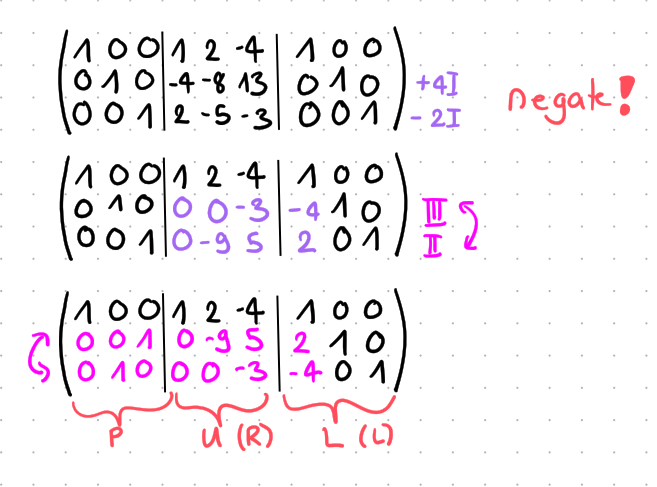
\includegraphics[scale=0.5]{pictures/LU-decomposition.png} 
\end{figure}

\mysection[JungleGreen]{\centering Vectorspaces}
\DEF{}{A vectorspace \COL{V} over $\mathbb{K}$ is a non-empty set, on which vectoraddition and scalarmultiplication is defined}
\DEF{Axioms}{\begin{itemize}
\item[V1]: $x+y=y+x$
\item[V2]: $(x+y)+z=x+(y+z)$
\item[V3]: $\exists 0 \in V: x+0=x$
\item[V4]: $\forall x \exists -x: x+(-x)=0 $
\item[V5]: $\alpha(x+y)=\alpha \cdot x+\alpha \cdot y$
\item[V6]: $(\alpha + \beta)x = \alpha x + \beta x$
\item[V7]: $(\alpha \beta)x=\alpha (\beta x)$
\item[V8]: $1\cdot x = x $
\end{itemize}}
\SA{4.1}{\begin{itemize}
\item[i]: $ 0 \cdot x = 0$
\item[ii] : $\alpga \cdot 0= 0 $
\item[iii]: $\alpha \cdot x =0 \rightarrow x=0 \vee \alpha = 0 $
\item[iv] : $(-\alpha)x = \alpha (-x)= -(\alpha \cdot x) $
\end{itemize}}
\DEF{polynomial space}{$\mathcal{P}_n$ is defined as all polynomials of degree $n$. Further: $ \mathcal{P} = \bigcup_{n=0}^{\infty} \mathcal{P}_n $}
\SA{4.1}{I a vectorspace the following holds for a scalar $\alpha $ and $x \in V $: \begin{itemize}
\item $ 0x = 0$
\item $ 0 \alpha = 0 $
\item $ \alpha x = 0 \Rightarrow \alpha = 0 $ or $x = 0 $
\item $ (-\alpha)x = \alpha(-x) = -(\alpha x) $
\end{itemize}}
\SA{4.12}{$\{ b_1 , \cdots , b_n\} \subset V$ is a basis of V $\Leftrightarrow $ every vector $x \in V$ can be uniquely represented as: $x = \sum_{k=1}^{n}\xi_k b_k $}
\SA{4.2}{$\forall x \in V, \forall y \in V \exists z \in V: x+z=y$ where $z$ is unique and $z = y + (-x) $}
\mysubsection{\centering Subspace}
\DEF{}{A subspace (unterraum) U is a non-empty subset of V. It is closed under vector addition and scalar multiplication. U contains the zero-vector}
\SA{4.3}{Every subspace is a vectorspace}




\DEF{spanning set}{The vectors $v_1 , \cdots , v_n$ are a spanning set (erzeugendes System) of V, if $\forall w \in span \{ v_1 , \cdots , v_n \} $ }

\mysubsection{\centering Linear dependency, basis, dimensions}
\DEF{linear dependency}{ Vectors $v_1 , \cdots , v_n$ are linearly dependent $\Leftrightarrow \sum_{k=1}^{n} \alpha_k \cdot v_k = 0 \rightarrow \alpha_1 = \cdots = \alpha_n = 0$}
\DEF{dimension}{ the dimension of V is $dim V = | span V|$ ($ dim\{0\}=0$)}
\LEM{4.8}{Every set $\{ v_1 , \cdots , v_m \} \subset V$ with $ |\mathbb{B}_v|<m$ is linear dependant }
\COR{4.10}{in an finite vectorspace, a set with $n$ independant vectors is basis of $V$ if $dim(V)=n$}
\DEF{}{The coefficients $\xi_k$ are coordinates of x with respect to a basis $\mathbb{B}$ $\xi = ( \xi_1 , \cdots , \xi_n )^T$ is a coordinate vector}
\DEF{}{Two subspaces $U, U' \subset V $ are complementary if every $ v \in V $ has a unique representation in $ U and U'$. Namely, $v = u \in U + u' \in U'$. $ \rightarrow V = U \bigoplus U'$}
\mysection[Aquamarine]{\centering Linear Maps}
\mysubsection{\centering Definitions}
\DEF{linearity}{$F: V\rightarrow W$ is linear:
\begin{itemize}
\item $F (v+w) = F(v)+F(w) $
\item $\alpha F(v) = F(\alpha v) $
\end{itemize}}
\DEF{injective}{$ \forall x, x' \subset X: f(x) = f(x') \Leftrightarrow x=x' $}
\DEF{surjective}{$ \forall y \subset Y, \exists x \subset X, f(x)=y $}
\DEF{bijective}{surjective and injective$ \Leftrightarrow f^{-1}$ exists}
\mysubsection{\centering Matrix representation}
Let F be a linear map $X \rightarrow Y$. One can write $F(b_i) \in Y$ as a linear combination of the basis of Y: $F(b_i) = \sum_{k=1}^{m} a_{k,l}\cdot c_k$ 
\DEF{}{The matrix $A^{m \times n}$ witht the elements $a_{k,l}$ is a matrix (Abbildungsmatrix) with respect $X,Y$}
$F(x)=y \Leftrightarrow A\xi = \eta $
\begin{Figure}[H]
 \centering
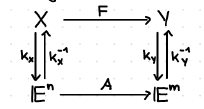
\includegraphics[width=\linewidth]{pictures/basistransformation.png}
\end{Figure}

\DEF{isomorphism}{F is bijective $\Leftrightarrow $ F is an isomorphism}
\DEF{automorphism}{F is isomorphism and $X = Y\Leftrightarrow $ F is an automorphism}
\SA{5.1}{F is isomorphism $\Leftrightarrow F^{-1}$ exists and is an isomorphism and linear}
\mysubsection{\centering Kernel, Image and Rank}

\DEF{Kern}{ $ ker F = \{ x \in X | F(x)=0 \}$}
\SA{5.6}{F injective $\Leftrightarrow ker F = \{0\} $}
\DEF{Image}{ $ Im F = \{ F(x) | x \in X \}$}
\SA{5.6}{F surjective $\Leftrightarrow im F = Y $}
\COL{ker A} is the solution set of $Ax=0$. \COL{$Im (A)$} set of all b, such that $Ax=b$ is solvable
\SA{5.7}{$dim X - dim (ker F) = dim (im F) = Rank(F) $}
\DEF{}{The rank F is equal to $dim(im (F))$}
\COR{5.8}{
\begin{itemize}
\item $F: X \mapsto Y $ injective $\Leftrightarrow $ Rank F = dim X
\item $F: X \mapsto Y $ surjective $\Leftrightarrow $ Rank F = dim Y
\item $F: X \mapsto Y $ bijective (isomorphism) $\Leftrightarrow $ Rank F = dim X = dim Y

\item $F: X \mapsto Y $ bijective (automorphism) $\Leftrightarrow $ Rank F = dim X, ker F $= \{0\}$
\end{itemize}

}
\COR{5.10}{\begin{itemize}
\item $Rank (G \circ F) \leq min(Rank F, Rank G)$
\item G is injective $Rank (G \circ F) = Rank F $
\item G is surjective $Rank (G \circ F) = Rank G $
\end{itemize}}
\mysubsection{\centering Matrices as linear mapping}
\DEF{columnspace}{ The columnspace (Spaltenraum) of $A$ is the subspace $\Re(A)= im(A)= span \{ a_1 , \cdots , a_n \} $}

\DEF{nullspace}{The nullspace (Nullraum) of A is a subspace $ \mathcal{N}(A) = ker A = L_0(Ax=0)$}

\DEF{}{\# free variables $=dim N(A) $}
\SA{5.12}{Rank A =r: and $L_0$ Solution of $Ax=0 \Rightarrow dim L_0 = dim N(A) = dim(Ker A)= n-r$}
\SA{5.13}{Rank $A \in M^{m \times n}$: 
\begin{itemize}
\item # pivots in Row-echelon-form
\item $dim(im (A))$ of $A: \mathbb{E}^n \mapsto \mathbb{E}^m $
\item dimension of the linear independent columns/rows
\end{itemize}}
\COR{5.14}{$Rank A^T= Rank A^H = Rank A$}
\SA{5.16}{for $A \in \mathbb{E}^{m \times n} $ and $B in  \mathbb{E}^{p \times m} $:
\begin{itemize}
\item $Rank BA \leq min (Rank A,Rank B)$
\item $Rank B  = m \leq p \Rightarrow Rank BA = Rank A$
\item $Rank A = m \leq n \Rightarrow Rank BA = Rank B$
\end{itemize}

}
\COR{5.17}{From S.5.16 it follows for quadratic matrices. $A \in \mathbb{E}^{m \times m} $ and $B in  \mathbb{E}^{m \times m} $
\begin{itemize}
\item $Rank BA \leq min (Rank A,Rank B)$
\item $Rank B  = m  \Rightarrow Rank BA = Rank A$
\item $Rank A = m  \Rightarrow Rank BA = Rank B$
\end{itemize}

}


}
\SA{5.18}{For quadratic matrix $\mathbb{E}^{n \times n}$ the following statements are equivalent:

\begin{itemize}
\item $A$ is regular
\item $Rank A = n$
\item Columns are linearly independent
\item Rows are linearly independent
\item $ker A = N(A)= \{0 \}$
\item $A$ is invertible
\item $Im A = \Re(A)= \mathbb{E}^n$
\end{itemize}



}
\SA{5.19}{For $Ax=b, b \neq 0$ with the solution $x_0$ and $L_0$ the solutionset is defined by $L_b = x_0 + L_0$ and is called \COL{affine subspace} (not a real subspace since $ 0 \notin L_b$)}
$ dim (Im (A)) = n - dim (ker (A)) = n - (n-r)=r$
\KRZ{Find Basis of Im A$ = \mathcal{R}(A) $}{
\begin{itemize}
\item[1] bring into row echelon form
\item[2] mark rows with pivots
\item[3] marked columns in the normal form are a Basis 
\end{itemize} \COL{ex} $ \begin{smallmatrix}
-1 & -4 &7  &3  \\
 3&  0&-6  &0  \\
 -3&4  & 1 &-3  \\
 1&-4  & 3 &3  \\
\end{smallmatrix}\xrightarrow[(1)]{} \begin{smallmatrix}
-1 & -4 &7  &3  \\
 0&  -12&15  &9  \\
 0&0  & 0 &0  \\
 0&0  & 0 &0  \\
\end{smallmatrix}\xrightarrow[(2)]{}\begin{smallmatrix}
-1 & -4 &7  &3  \\
 \uparrow &  -12&15  &9  \\
 0& \uparrow  & 0  &0  \\
 0&0  & 0 &0  \\
\end{smallmatrix}\xrightarrow[(3)]{} span \left\{ \begin{smallmatrix}
-1 \\
3 \\
 -3\\
1\\
\end{smallmatrix}   \begin{smallmatrix}
-4 \\
0 \\
 4\\
-4\\
\end{smallmatrix} \right\} $}

\KRZ{Find Basis of ker A $ = \mathcal{N}(A), A \in E^{m \times n}$}{
\begin{itemize}
\item[1] bring into row echelon form
\item[2] create a vector for every row, which does not have a pivot. The dimensions of the vectors are $E^{1 \times n}$ 
\iten[3]Solve SLE $Ax=0$ with the yielded vectors.
\item[4]  Write the solution as vector
\end{itemize} \COL{ex} $ \begin{smallmatrix}
-1 & -4 &7  &3  \\
 3&  0&-6  &0  \\
 -3&4  & 1 &-3  \\
 1&-4  & 3 &3  \\
\end{smallmatrix}\xrightarrow[(1)]{} \begin{smallmatrix}
-1 & -4 &7  &3  \\
 0&  -12&15  &9  \\
 0&0  & 0 &0  \\
 0&0  & 0 &0  \\
\end{smallmatrix}\xrightarrow[(2)]{}\begin{smallmatrix}
-1 & -4 &7  &3  \\
0 &  -12&15  &9  \\
 0& 0  & \uparrow   &\uparrow   \\
 0&0  & 0 &0  \\
\end{smallmatrix}\xrightarrow[(3)]{} \begin{smallmatrix}
x_4 = \alpha \\
x_3 = \beta \\
x_2 = \frac{5\beta+3\alpha}{4}\\
x_1 = 2\alpha
\end{smallmatrix}


\xrightarrow[(4)]{}

span \left\{ \begin{smallmatrix}
2 \\
\frac{5}{4} \\
1\\
0\\
\end{smallmatrix}   \begin{smallmatrix}
0 \\
\frac{3}{4} \\
 0\\
1\\
\end{smallmatrix} \right\} $}
\DEF{Maps}{Let $X,Y$ be vector spaces with $dim X = n, dim Y = m$
\begin{itemize}
\item $F: X \mapsto Y$ a linear map
\item $A: \mathbb{E}^n \mapsto \mathbb{E}^m',\xi \mapsto \eta $ *

\item $B: \mathbb{E}^n \mapsto \mathbb{E}^m,\xi' \mapsto \eta' $ *
\item $T: \mathbb{E}^n \mapsto \mathbb{E}^n',\xi \mapsto \xi' $ **
\item $S: \mathbb{E}^m \mapsto \mathbb{E}^m',\eta \mapsto \eta' $** 
\end{itemize}
}
*Abbildungsmatrix\\
**Transformationsmatrix

\begin{Figure}
 \centering
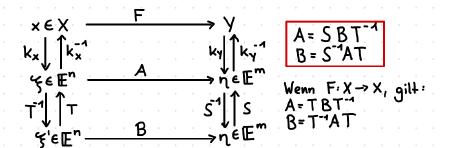
\includegraphics[scale=1]{pictures/transform.png} 
\end{Figure}

\SA{5.20}{$Rank F = r $ has the mappingmatrix* $A =  \left[ 
\begin{array}{c|c} 
  I_r &0 \\ 
  \hline 
  0 & 0
\end{array} 
\right]  $}


\mysection[RoyalBlue]{\centering Vector spaces with scalar products}

\mysubsection{\centering Definitions}
\DEF{Norm}{A norm is a function $|\cdot|:V\rightarrow \mathbb{R}, x \rightarrow \left\|x \right\| $ in a vector space which satisfies: \begin{itemize}

\item[N1] $ \left\|x \right\| > 0 , \left\|x \right\| = 0 \Leftrightarrow x=0$ (positiv definit)
\item[N2] $\left\|\alpha x \right\| = \alpha \left\|x \right\| $ (homogenous)
\item[N3] $\left\|x \pm y \right\| \leq \left\|x \right\| + \left\|y \right\|$ (Triangle-inequality)
\end{itemize}} 
A \COL{normed vector space} has a norm
\DEF{scalar product}{is a function $\left< \cdot,\cdot \right>: V \times V \rightarrow \mathbb{E}, x,y \mapsto\left< x,y\right>  $, which satisfies:
\begin{itemize}

\item[S1] $ \left< x,y+z\right>=\left< x,y\right>+\left< x,z\right> $(linear in 2nd factor)
\item[S1] $ \left< x,\alpha y\right> = \alpha\left< x,y\right>$ (linear in 2nd factor)
\item[S2] $ \left< x,y\right>=\overline{\left< x,y\right>}$(symmetric, hermitian)
\item[S3] $ \left< x,x\right> > 0, \left< x,x\right>=0\Leftrightarrow x=0$(positiv definite))
 
\end{itemize}



}
\DEF{unitsphere}{the set $\{ x \in V |\left\|x\right\| =1 \}$}
\DEF{induced norm}{The length of a vector is defined as: $\left\| \cdot \right\|: V \mapsto \mathbb{R}, \left\|x\right\|  \mapsto \sqrt{\left< x,x\right>}  $}
\DEF{angle  $\phi $}{$\phi = \sphericalangle(x,y) , 0 \leq \phi \leq \pi $ is defined by: $\phi = \frac{\left< x,x\right>}{\left\| x \right\| \cdot \left\| y \right\|}=\frac{\Re \left< x,y\right>}{\left\| x \right\| \cdot \left\| y \right\|} $}

\DEF{orthogonal vectors}{two vectors $x,y$ are orthogonal $\Leftrightarrow \left< x,y\right> = 0  $}
\DEF{orthogonal sets }{two sets $X,Y$ are orthogonal $\Leftrightarrow  \forall x \in X, \forall y \in Y \left< x,y\right> = 0  $}
\SA{6.1}{$ \left| \left< x,y \right> \right|^2 \leq  \left< x,x \right>  \left< y,y \right> = \left\| x\right\|^2 \cdot \left\| y\right\|^2$(Cauchy Schwarz Inequality)}
\SA{6.2}{$\left\|x \pm y \right\|^2 = \left\|x \right\|^2 + \left\|y \right\|^2 \Leftrightarrow x \perp  y  $(Pythagoras)}
\DEF{orthogonal basis}{ $\Leftrightarrow \forall i, \forall j, i \neq j: \left< b_i,b_j \right>  = 0  $}
\DEF{orthonormal basis}{ $\Leftrightarrow $ orthogonal basis with vectors of length 1}
\SA{6.3}{A set $M$ of pairwise orthogonal vectors are linearly independant if $0 \notin M $}
\SA{6.4}{Let $\{ b_1, \cdots , \b_n \}$ a orthonormal basis, $x \in V$: $x = \sum_{k=1}^{n} \left< b_k,x \right>b_k \rightarrow \xi_k = \left< b_l,x \right> $ }
\SA{6.5}{from $ \xi_k = \left< b_l,x \right>_v, \eta_k = \left< b_l,x \right>_v$ follows $ \left< x,y\right>_v = \sum_{k=1}^{n} \overline{\xi_n} \eta_k = \xi^H \eta = \left< \xi,\eta \right>_{\mathbb{E}^n} $ Which implies that if a basis in $V$ is orthonormal the scalar product is valid in $V$}
From that follows: $ \left\| x\right\|_v= \left\| \xi\right\|_{\mathbb{E}^n}, \sphericalangle (x,y)_v = \sphericalangle (\xi, \eta)_{\mathbb{E}^n}, x \perp y \Leftrightarrow \xi \perp \eta$
\KRZ{Gram-Schmidt}{\begin{itemize}
\item $b_1 = \frac{a_1}{\left\| a_1\right\|_v}$
\item $\widetilde{b_k} = a_k -\sum_{j=1}^{k-1} \left< b_j,a_k\right>_v \cdot b_j $
\item $b_k = \frac{\widetilde{b_k}}{\left\| \widetilde{b_k}\right\|_v} $
\end{itemize} \COL{ex } $ A= \begin{smallmatrix}
2 &3  \\
 2&4  \\
 1&1  \\
\end{smallmatrix}\xrightarrow[1]{}a_1 = \begin{smallmatrix}
 2\\
 2\\
1
\end{smallmatrix} / \left\| \begin{smallmatrix}
 2\\
 2\\
1
\end{smallmatrix}  \right\|= \begin{smallmatrix}
 2/3\\
 2/3\\
1/3
\end{smallmatrix}, \widetilde{a_2} = \begin{smallmatrix}
 3\\
 4\\
1
\end{smallmatrix} - \left<  \begin{smallmatrix}
 2/3\\
 2/3\\
1/3
\end{smallmatrix}, \begin{smallmatrix}
 3\\
 4\\
1
\end{smallmatrix}\right> = \begin{smallmatrix}
 -1/3\\
 2/3\\
-2/3
\end{smallmatrix}, a_2 = \begin{smallmatrix}
 -1/3\\
 2/3\\
-2/3
\end{smallmatrix} /\left\|\begin{smallmatrix}
 -1/3\\
 2/3\\
-2/3
\end{smallmatrix} \right\| = \begin{smallmatrix}
 -1/3\\
 2/3\\
-2/3
\end{smallmatrix} \mapsto A = \begin{smallmatrix}
 2/3& -1/3  \\
 2/3& 2/3 \\
2/3 & -2/3 \\
\end{smallmatrix} $}
\SA{6.6}{After k-steps the set $\{b_1, \cdots , b_k \}$ is pairwise orthonormal.$\{b_1, \cdots , b_k \} \text{ is a basis} \Leftrightarrow \{a_1, \cdots , a_k \} \text{ is a basis}$ Every vectorspace ($\neq \infty$) has a orthonormal basis }
\COR{6.7}{To a vector space with scalar product with finite or countably infinite many dimensions a orthonormal basis exists.}
\DEF{orthogonal complement}{$U^\perp$ is the orthogonal complement of a subspace $U$. $U \bigoplus  U^\perp = V $}
\SA{6.9}{For a complex matrix with $rank A = r$ it holds: \begin{itemize}
\item $N(A)= \Re(A^H)^{\perp} \subset \mathbb{E}^n $
\item $N(A^H)= \Re(A)^{\perp} \subset \mathbb{E}^m $
\item $N(A) \bigoplus \Re(A^H) = \mathbb{E}^n $
\item $N(A^H) \bigoplus \Re(A) = \mathbb{E}^m $
\item $dim \Re(A)= r$
\item $dim \Re(A^H)= r$
\item $dim N(A)= n-r$
\item $dim N(A^H)= m-r$
\end{itemize}


} Those  are the \COL{fundamental subspaces}
\mysubsection{\centering Change of Basis}
$\mathcal{B},\mathcal{B}' $ are orthonormalbasis. Hence: $b_k' = \sum_{n}^{j=1} \mathcal{T}_{jk}b_j$ Matrix for change of basis $T$: $T^{-1} = T^H $ since both basis are orthonormal. Therfore it holds that:
\begin{itemize}
\item $\xi = T\xi'$
\item $\xi' = T^{-1}\xi$
\item $\mathcal{B} = ,\mathcal{B}'T$
\item $\mathcal{B}' = ,\mathcal{B}T^{H}$
\end{itemize}
\SA{4.13}{Let \textbf{$\xi $}$= (\xi_1  \cdots \xi_n)^T $ be a coordinate  vector of an arbitrary vector $v \in V$ with respect to the \COL{old basis}. Let \textbf{$\xi $}'$= (\xi_1'  \cdots \xi_n')^T $ be the new representation of a vector $x$ with respect to the new basis. $x = \sum_{i=1}^{n}\xi_i b_i = \sum_{k=1}^{n}\xi_k' b_k' $}
All matrices are unitary/orthogonal
\COR{6.12}{$\left< x,y \right>_v  = \xi^H \eta =\left< \xi,\eta \right>_v = \left< \xi',\eta' \right>_v = \xi'^H \eta' \Rightarrow T$ is conformal (längen-winkeltreu)}


\NOTE{Convention}{
A representation of a vector with respect ot the basis $\mathcal{B}_1$ is written as $[v]_{\mathcal{B}_1}$ \\
Therefore:
$[v]_{\mathcal{B}_2} = Mat(\mathcal{B}_1)_{\mathcal{B}_2}[v]_{\mathcal{B}_1}$ and $ [v]_{\mathcal{B}_1} = Mat(\mathcal{B}_2)_{\mathcal{B}_1}[v]_{\mathcal{B}_2}$ where $Mat(\mathcal{B}_2)_{\mathcal{B}_1}$ is the matrix of change ob basis \textbf{from} $\mathcal{B}_1 $ \textbf{to} $\mathcal{B}_1 $ Hence: $Mat(\mathcal{B}_1)_{\mathcal{B}_2} = \begin{pmatrix}
[b_1]_{\mathcal{B}_2}&\left| \cdots\right|   & [b_n]_{\mathcal{B}_2} \\
\end{pmatrix}  $}

\KRZ{Calculating the matrix of $F$ with respect to Basis $\mathcal{B} $: We have a function $F: X \mapsto X$ and the basis of X $:=\mathcal{B} $}{

\begin{itemize}
\item[1] calculate for all $\forall a \in \mathcal{B}$: $F(b_a) $ 
\item[2] solve for all $F(b_a) = \alpha_a b_1 + \beta_a b_2 \cdots \gamma_a b_n $
\item[3] write coordinate vectors as: $ \xi_a = (\alpha_a \beta_a \cdots \gamma_a)^T$
\item[4] write matrix as $F_{[\mathcal{B}]} =  \begin{smallmatrix}
\xi_1 &
\left| \cdots \right|  &
 \xi_n &
\end{smallmatrix}$ 
\end{itemize}}


\KRZ{Compute Basistransformationsmatrix from $\mathcal{B} $ to $\mathcal{S} $ }{
Since $\mathcal{S} $ is a standardbasis we have: 
\begin{itemize}
\item[1] $\mathcal{S} \rightarrow \mathcal{B} $ is given by $B   = (s_1 | s_2 | \cdots | s_n)$ (Columns of $B$ are the basis vectors of $\mathcal{B}  $)
\item[2] Compute inverse of $B$ to get $\mathcal{B} \rightarrow \mathcal{S}   $
\end{itemize}
}

 \KRZ{Basistransformationsmatrix from $2\times 2 $ matrices with respect to the standard basis}{
 The standard basis of $2\times 2 $ matrices is given by: $ \mathcal{S} = \left\{\begin{pmatrix}
1 &0  \\
 0& 0 \\
\end{pmatrix}, \begin{pmatrix}
0 &1  \\
 0& 0 \\
\end{pmatrix}, \begin{pmatrix}
0 &0  \\
 1& 0 \\
\end{pmatrix} ,\begin{pmatrix}
0 &0  \\
 0& 1 \\
\end{pmatrix}\right\} $ and the new Basis is defined by: $\mathcal{B} = \left\{\begin{pmatrix}
a &b  \\
 c& e \\
\end{pmatrix}, \begin{pmatrix}
e &f  \\
 g& h \\
\end{pmatrix}, \begin{pmatrix}
i &j  \\
 k& l \\
\end{pmatrix} ,\begin{pmatrix}
m &n  \\
 o& p \\
\end{pmatrix}\right\} $ Then the matrix (Abbildungsmatrix) is defined by $F = \begin{pmatrix}
a & e & i  & m  \\
b & f & j  & n \\
c & g & k & o \\
d & h &  l & p \\
\end{pmatrix} $
 
 }

\KRZ{Prove that $\mathcal{B} $ is Basis}{
$\mathcal{S} $ denotes the standard basis.

\begin{itemize}
\item[1]  compute for all $\forall a \in \mathcal{B}$: $b_a = \alpha s_1 + \beta s_2 \cdots \gamma s_n $ 
\item[2] Since $span(\mathcal{B}) = span(\mathcal{S}) $, $\mathcal{B}$ has to be basis.
\end{itemize}}


\KRZ{Prove that $F$ is a bijective mapping $F: X \mapsto Y$ with the basis $\mathcal{X}$ for $X$ and  $\mathcal{Y}$ for $Y $ }{

\begin{itemize}
\item[1] calculate for all $\forall a \in \mathcal{X}$: $F(x_a) $
\item[2] solve for all $F(x_a) = \alpha_a y_1 + \beta_a y_2 \cdots \gamma_a y_n $
\item[3] write coordinate vectors as: $ \xi_a = (\alpha_a \beta_a \cdots \gamma_a)^T$
\item[4] write matrix as $F_{[\mathcal{X}]} =  \begin{smallmatrix}
\xi_1 &
\left| \cdots \right|  &
 \xi_n &
\end{smallmatrix}$ 
\item[5] As $F_{[\mathcal{X}]} $ is quadratic and has full rank we have that $dim( \mathcal{X})  = dim( \mathcal{Y})$ and thus by Cor.5.8 that F is bijective
\end{itemize}}





\mysubsection{\centering unitary/orthogonal mapping}
\DEF{unitary}{A linear mapping$F: X \mapsto Y$ is unitary/orthogonal if $ \left< F(v),F(w)\right>_y = \left< v,w\right>_x$}
\SA{6.13}{\begin{itemize}
\item[1] $F$ is isometric (längentreu): $\left\| F(v)\right\|_y= \left\| v\right\|_X $
\item[2] $F$ is conformal (winkeltreu): $v \perp w \Leftrightarrow F(v) \perp F(w) $
\item[3] $ker F = \{0\}$, F is injective
\item if $n = dim X = dim Y < \infty$
\item[4] $F$ is isomorphism
\item[5] $\{ b_1, \cdots ,b_n \} $ is orthonormal basis of X $\Leftrightarrow \{ F(b_1), \cdots ,F(b_n) \}$ is a orthonormal basis of Y
\item[6] $F^{-1} $ is unitary/orthogonal
\item[7] The mapping matrix (Abbildungsmatrix) A is  unitary/orthogonal
\end{itemize}}
\mysection[Plum]{\centering Least Squares}
Let $Ax=b$ a overdetermined SLE (# Equations > #Variables). No exact solution exists. $\rightarrow x^* = argmin_{x \in \mathbb{E}^n}  \left\| Ax-b\right\|_2^2  \Rightarrow (Ax-b)\perp \Re(A)$

\DEF{Pseudoinverse}{If Rank A = n: $A^+= (A^HA)^{-1}A^H \Rightarrow A^+A=I $}
\DEF{normalequations}{$ (A^TA)x = A^Ty  $}
\KRZ{Least Square Method for functions}{We assume that $ ker(A)=\{0\}$ and $A^HA $ is regular
\begin{itemize}
\item[0] bring problem in a form where everything is numerically determined except the coefficients
\item[1] calculate $A^Ty $
\item[2] calculate $A^TA $
\item[3] solve the equation $(A^TA)x = A^Ty $ 
\item[4] calculate error $r = y-Ax $
\end{itemize}
\COL{ex} The equation is given $y(t)= x_1 t + x_2t^2 $ We have $t_n (1,2,3,4)$ and $y(t)_n = (13.0,35.5,68.0,110.5)$
$\xrightarrow[0]{}A=\begin{smallmatrix}
 1&  1\\
 2& 4 \\
 3& 9 \\
4 &  16\\
\end{smallmatrix}, y = \begin{smallmatrix}
 13.0\\
 35.5\\
 68.0 \\
110.5 \\
\end{smallmatrix} \xrightarrow[1]{} A^Ty = \begin{smallmatrix}
730.0 \\ 2535.0 \end{smallmatrix} \xrightarrow[2]{} A^TA = \begin{smallmatrix}
 30&  100\\
100 &  354\\

\end{smallmatrix}\xrightarrow[3]{}\left.\begin{smallmatrix}
30 & 100 \\
 100& 354 \\
\end{smallmatrix}\right|\begin{smallmatrix}
 730\\2535.0
\end{smallmatrix}\mapsto x_1 = 7.9355, x_2 = 4.919 $}






\KRZ{Least Square Method for 2D-points}{
\begin{itemize}
\item[0] Write X- / Y-coordinate alternately in the form $(x , 0)$, $(0,y)$ in $A$ for every point.  Write X- / Y-coordinate alternately in y.
\item[1] Rest as usually
\end{itemize}
\COL{ex} The points $P = \left\{(-1,1),(1,1),(1,-1),(-1,-1) \right\}$ should be transformed with respect to the squared distance to the points $P' = \left\{(0,2),(1,3),(0,-2),(-1,-3) \right\}$. The transformation is defined as $T(P) = T \left ( \begin{smallmatrix}
 p_x\\p_y
\end{smallmatrix} \right ) = \left ( \begin{smallmatrix}
 s_x \cdot p_x\\s_y \cdot p_y
\end{smallmatrix} \right ) $

 $Ax = y \Rightarrow \begin{pmatrix}
 -1&0  \\
 0&1  \\
 1&0  \\
 0& 1 \\
 1&0  \\
 0&-1  \\
 -1&0  \\
 0& -1 \\
\end{pmatrix} \begin{pmatrix}
s_x \\ s_y
\end{pmatrix} = \begin{pmatrix}
 0\\
 2\\
 1\\
3 \\
0 \\
-2 \\
-1 \\
-3
\end{pmatrix}$

}




\KRZ{Least Squares with QR-decomposition}{We have the normal equations $A^HAx = A^Tb \Rightarrow (QR)^H (QR)x = (QR)^H b \Rightarrow R^HQ^H QRx= R^HQ^H \Rightarrow R^HRx = R^TQ^Tb \Rightarrow Rx = Q^Hb$ Therefore we have: \begin{itemize}
\item[1] compute QR-decomposition of A
\item[2] solve $Rx = Q^Tb$
\end{itemize}}



\KRZ{Least Squares with SVD}{$\left\| Ax-b \right\|_{2}^2 = \left\| \Sigma \underbrace{V^{H}_x}_{y} - \underbrace{U^H b}_{c} \right\|_{2}^2 = \left\| \Sigma y - c \right\|_{2}^2 $;$x^* = V \Sigma^{+}U^H b \Rightarrow \infty $ solutions, here: smallest 2-norm ($y^* = \Sigma^{+}U^H b $) Where $\Sigma^{+} $ is the pseudoinverse of $\Sigma $, hence it holds}
\mysection[Orchid]{\centering Determinants}
\DEF{}{$det\left ( a_{11} \right ) = a_{11}, det\begin{pmatrix}
a_{11} &a_{12}  \\
a_{21} & a_{22} \\
\end{pmatrix} = a_{11}a_{22}-a_{12}a_{21}$,\\$det\begin{pmatrix}
a_{11} & a_{12} &a_{13}  \\
a_{21} &a_{22}  & a_{23} \\
 a_{31}&a_{32}  &a_{33}  \\
\end{pmatrix} = \begin{matrix}
a_{11}a_{22}a_{33}    & + a_{21}a_{32}a_{13}\\
+a_{31}a_{12}a_{23}   & - a_{13}a_{22}a_{31}  \\
- a_{12}a_{21}a_{33}    &-  a_{11}a_{23}a_{32}  \\
\end{matrix} $}
\SA{8.12}{$det (A) = \sum_{i=1}^{n}a_{ki}\mathcal{K}_{ki} = \sum_{i=1}^{n}a_{il}\mathcal{K}_{il} $ for a fixed $k$ and $l$.}
\DEF{cofactor $\mathcal{K}_{ki} $}{$\mathcal{K}_{ki}  = (-1)^{k+i} det(A_{\left [ k,i \right ]})}$}
\DEF{ $A_{\left [ k,i \right ]}$}{Is defined as the matrix $A$ without the $k-th$ row and $i-th$ column }
\DEF{}{$det A = 0 \Leftrightarrow A $ is singular}
\DEF{}{$det A \neq 0 \Leftrightarrow A $ is regular}
\SA{8.3}{
\begin{itemize}
\item[i] $det(A)$ is linear in every row
\item[ii] swapping two rows changes the sign of  $det(A)$ 
\item[iii]  $det(I)=1$ 
\end{itemize}}
\SA{8.4}{\begin{itemize}
\item[iv] if A has a row with 0 $\Rightarrow det(A)=0$
\item[v] $det(\gamma A) = \gamma^n det(A)$
\item[vi] if A has to equal rows  $\Rightarrow det(A)=0$
\item[vii] adding a multiple of a row to another row doesnt affect the det
\item[viii] is A a diagonalmatrix: $det(A)=\prod_{i=1}^{n}a_{ii} $
\item[iv] is A a triangularmatrix: $det(A)=\prod_{i=1}^{n}a_{ii} $
\end{itemize}}
\COR{8.10}{Every statement of Satz 8.3 and 8.4 also holds for columns instead of rows}



\SA{8.5}{Using Gauss on A results in: $det(A) = (-1)^v \prod_{k=1}^{n}r_{kk} $} where $v$ is \# swappings of rows and $r_{kk}$ are the diagonal elements of the row echelon form
\SA{8.7}{$det(AB)=det(A)\cdot det(B)$}
\COR{8.8}{if A is regular $\Rightarrow det (A^{-1})= \frac{1}{det(A)} $}
\SA{8.9}{$det(A^T)=det(A) $ and $det(A^H)=\overline{det(A)} $}
\DEF{det of block matrices}{$det \left[ 
\begin{array}{c|c} 
  A & C \\ 
  \hline 
  0 & B
\end{array} 
\right]  = det (A)\cdot det(B)$}
\DEF{det of unitary matrices}{Let $A $ be unitary/orthogonal $ |det(A)|=\pm 1 $ proof: $det(U^TU) = det(I)= (det(U))^2 = 1 \Rightarrow det(U)= \pm 1 $}
\mysection[Magenta]{\centering Eigenvalues and -vectors}
\DEF{eigenvector}{A number $\lambda \in \mathbb{E}^n$ is called eigenwert of a linear mapping: $F: X\mapstoX$ if $\exists v \in V, v \neq 0$ such that $F(v) = \lambda v$. v is an eigenvector. The set of all eingenvectors, which corespond to $\lambda$ form a subspace $E_{\lambda} = \{ v \in V |F(v) = \lambda v \}$}
\DEF{spectrum}{The set of all eigenvalues of F is called spectrum}
\DEF{}{$\xi \in \mathbb{E}^n$ is a eigenvector of $\lambda \Leftrightarrow A\xi = \lambda \xi$}
\LEM{9.1}{A linear map $F$ and its matrix representation have the same eigenvalues and the eigenvectors are connected by the coordinaterepresentation $k_v$}
\LEM{9.2}{$\lambda $ is eigenvalue $\Leftrightarrow ker(A-\lambda I) $ is singular ($E_{\lambda} = ker(A-\lambda I) $)}
\DEF{multiplicity}{The geometric multiplicity of $\lambda  = dim (E_{\lambda})$ }
\DEF{characteristic polynomial}{It is defined by $ \mathcal{X}_A(\lambda)= det(A-\lambda I)=0$}
\DEF{Trace}{$tr(A) = \sum_{k=1}^{n}a_{kk} $ }
\SA{9.5}{$\lambda \in \mathbb{E}$ is eigenvalue of A $\Leftrightarrow \mathcal{X}_A(\lambda)=0$}
\LEM{9.4}{$ \mathcal{X}_A(\lambda)= (-1)^{n}\cdot \lambda^{n} (-1)^{n-1}\cdot tr(A) \cdot \lambda^{n-1} + \cdots det(A)\lambda^0 = a_n \cdot^n + a_{n-1}\cdot  \lambda^{n-1} + \cdots det(A)$}
\LEM{9.6}{A (quadratic) matrix is singular if and only if it has 0 as an eigenvalue}
\DEF{algebraic multiplicity}{ is the  multiplicity of an eigenvalue in the char. polynomial.}
\SA{9.13}{geometric multiplicity $\leq $ algebraic multiplicity}
\KRZ{Find Eigenvalues and -vectors}{\begin{itemize}
\item[1] find char. polynomial $\mathcal{X}_A(\lambda)= det(A-\lambda I) $
\item[2] find roots of $\mathcal{X}_A$ 
\item[3] for every $\lambda_k $ find the solution for $(A-\lambda_k I)x=0 $
\end{itemize}}
\SA{9.7}{for similar matrices $C = T^{-1}AT $ ($C$ and $A$ are similar) holds that $tr(A)=tr(C), det(A)=det(C), \mathcal{X}_A = \mathcal{X}_C$ and they have the same eigenvalues}
\SA{9.11}{Eigenvectors for different Eigenvalues are linearly independant $ \Rightarrow $ max $dimV$ different Eigenvalues }
\DEF{}{$ \lambda $ is eigenvalue for $A \Rightarrow \lambda^{q}$ is eigenvalue of $A^q$ }
\NOTE{Trace}{ $trace(A)$ is equal to the sum of all eigenvalues of $A$:$trace(A) = \lambda_1 +\cdots +\lambda_n$ }

\NOTE{Trace}{ $det(A)$ is equal to the producct of all eigenvalues of $A$:$det(A) = \lambda_1 \cdot \cdots \cdot \lambda_n$}

\mysection[WildStrawberry]{\centering Decompositions}
\mysubsection{\centering Spectral-/Eigenvaluedecomposition}


\DEF{}{$A = V \Lambda V^{-1 }$ ($A$ and $\Lambda$ are similar)}
Precondition for \COL{diagonalisation}:
\SA{9.14}{$A \in \mathbb{C}^{n \times n}$ is diagonalisible $ \Leftrightarrow \forall $ Eigenvalues (geom. mult. = alg. mult.)}
\SA{9.15}{If $A  \in \mathbb{C}^{n \times n} $ is unitary ($ A^H=A$)it holds that: \begin{itemize}
\item[i] all eigenvalues are real
\item[ii]  the eigenvectors are pairwise orthogonal
\item[iii] an orthonormal basis $U$ exists, which consists of all the eigenvectors
\item[iv] for the unitary matrix $U$ holds that  $U^HAU=\Lambda$  
\end{itemize}}
\COR{9.16}{The previous statements is also valid for real-symmetric matrices}




\KRZ{Eigenvaluedecomposition}{
\begin{itemize}
\item[1] find the eigenvalues of A $\lambda_k $ and write $\Lambda = diag(\lambda_1 \cdots \lambda_n) $
\item[2] find the according eigenvectors $v_k $ of  $\lambda_k$ write  them as $V = (v_1|\cdots|v_n) $ (sorted according to $\Lambda $) 
\item[3] find inverse $V^{-1} $
\end{itemize}}





\COR{9.10}{If $A$ is diagonisable it can be composed as a sum of \COL{1-rank-matrices}: $ A = \sum_{k=1}^{n}V_k \lambda_k w_k^T $ with $V = (V_1 \cdots V_n) $ and $V^{-1} = \begin{pmatrix}
 w_1^T\\
 \vdots \\
 w_n^T
\end{pmatrix} $ from that follows: $Av_k = v_k \lambda_k $ and $ w^T_k A = \lambda_k w^T_k$: $w^T  $ is a \COL{left eigenvector}}



\KRZ{Eigenvaluedecomposition with SVD}{ The SVD is given by $A = U \Sigma V^H$
\begin{itemize}
\item[1]  Expand $U \Sigma V^H \Rightarrow U I \Sigma V^H  \Rightarrow U I_{1} I_{2} \Sigma V^H $ where $U I_{1} = V $ and  $I_{1} I_{2} = I $
\item[2] Calculate $
\left ( U I_{1}  \right ) \left (I_{2} \Sigma  \right ) V^H  $
\end{itemize}

} 


\KRZ{Composition of 1-rank- matrices}{
\begin{itemize}
\item[1] write $A = V \Lambda V^{-1 }$
\item[2] rewrite $ A = \sum_{k=1}^{n}V_k \lambda_k w_k^T $
\textit{$V_k $ = row ($\downarrow $) of $V$, $w_k^T $ = column ($\rightarrow $) of $V^{-1} $ }
\end{itemize}
}


}

\KRZ{Powers of $A$}{

\begin{itemize}
\item[1] write $A = V \Lambda V^{-1 }$ 
\item[2] calculate $A^m = V \Lambda^m V^{-1 }$
\end{itemize}
note: $\Lambda^m = diag(a_{11}^m , \cdots , a_{nn}^m)$

}

\mysubsection{\centering Singularvaluedecomposition}
\DEF{SVD for $A^HA $}{Spectral-decomposition exists for every matrix $A^HA $. Since $A^HA $ is hermetian (hermetisch) and positive semidefinite.$\rightarrow $ $A^HA $ has real, non-negative eigenvalues $\lambda \in \mathbb{R} $ and $\lambda \geq 0 $ Therefore one can rewrite:$A^HAV = V\Lambda \xrightarrow[\lambda = \sigma ^2]{} A^HAV_r = V_r \Sigma_{r}^{2}\Rightarrow V_{r}^H A^HAV_r = \Sigma_{r}^{2} \Rightarrow \underbrace{(\Sigma_{r}^{-1} V_{r}^H A^H )}_{=U_{r}^{-1}}\underbrace{(AV_r \Sigma_{r}^{-1} )}_{=U_{r}}=I $  }

\DEF{SVD}{SVD exists for every matrix, such that $U,V$ are unitary and $\Sigma $ is diagonal and positive. $A = U \Sigma V^H $ it follows $AA^H =U\Sigma_{m}^2 U^H $,$A^H A=V \Sigma_{n}^2 V^H $, $A^H = V \Sigma^T U^H $}
\DEF{A invertible}{If A is invertible $A^{-1} = V \Sigma^{-1}U^H $}
\SA{11.11f}{For Rank $r$ it holds that: \begin{itemize}
\item $\{ u_1, \dots, u_1 \}$: Basis of $Im(A) = \mathcal{R}(A) $ 
\item $\{ u_{r+1}, \dots, u_m \}$: Basis of $Ker(A^H) = \mathcal{N}(A^H) $  
\item $\{ v_1, \dots, v_1 \}$: Basis of $Im(A^H) = \mathcal{R}(A^H) $ 
\item $\{ v_{r+1}, \dots, v_m \}$: Basis of $Ker(A) = \mathcal{N}(A) $  
\end{itemize}}
\DEF{Automorphism}{In a self-image (Selbstabbildung) it holds that $A = U \Sigma V^H = V \underbrace{V^HU}_{R}\Sigma V^H= \underbrace{V}_{1}\underbrace{R}_{2}\underbrace{\Sigma}_{3}\underbrace{V^H}_{4} $ \begin{itemize}
\item[1,4]  Change to orthonormal basis
\item[2] rotation, mirroring
\item[3] scaling of unit-axes
\end{itemize}}
\DEF{singular values}{singular values: $\sigma_i = \sqrt{\lambda_i} $ sorted in descending order $\sigma_a \leq \sigma_b \cdots \sigma_r \leq 0 \cdots  $ }
\DEF{Eigenbasis}{$V $ is the orthonormal eigenbasis of $A^HA $ such that: $AA^H =U\Sigma_{m}^2 U^H $. Similar for $U $ as eigenbasis of $AA^H $: $A^H A=V \Sigma_{n}^2 V^H $} 
\KRZ{SVD of $A \in \mathbb{E}^{m \times n}$with $A^HA $}{\begin{itemize}
\item[1] Calculate $(A^HA)\in \mathbb{E}^{n \times n}$
\item[2] find eigenvalue of $A^HA$
 \item[3] write $\Sigma_r = diag(\sqrt{\lambda_{1}}, \cdots, \sqrt{\lambda_{n}}) \in \mathbb{E}^{n \times n}$
\item[4] rewrite: $\Sigma \in \mathbb{E}^{m \times n} $: $\Sigma = \begin{smallmatrix}
 \Sigma_r&  0\\
 0& 0 \\
\end{smallmatrix}$
\item[5] find eigenvectors of $A^HA \Rightarrow v_1 ,\cdots ,v_r$
\item[6] norm eigenvectors and compute $V = ( \frac{v_1}{\left\| v_1 \right\|}|\cdots| \frac{v_n}{\left\| v_n \right\|}) \in \mathbb{R}^{n \times n} $
\item[7] solve for $U = AV\Sigma^{-1} $
\item[8] if $U_r \neq U$: $U_r \xrightarrow[gram]{schmidt} U \in \mathbb{E}^{m \times m} $
\item[9] write $A = U \Sigma V^H $
\end{itemize}}


\KRZ{SVD of $A \in \mathbb{E}^{m \times n}$with $AA^H $}{\begin{itemize}
\item[1] Calculate $(AA^H)\in \mathbb{E}^{m \times m}$
\item[2] find eigenvalue of $AA^H$
 \item[3] write $\Sigma_r = diag(\sqrt{\lambda_{1}}, \cdots, \sqrt{\lambda_{n}}) \in \mathbb{E}^{m \times m}$
\item[4] rewrite: $\Sigma \in \mathbb{E}^{m \times n} $: $\Sigma = \begin{smallmatrix}
 \Sigma_r&  0\\
 0& 0 \\
\end{smallmatrix}$
\item[5] find eigenvectors of $AA^H \Rightarrow v_1 ,\cdots ,v_r$
\item[6] norm eigenvectors and compute $V = ( \frac{v_1}{\left\| v_1 \right\|}|\cdots| \frac{v_n}{\left\| v_n \right\|}) \in \mathbb{R}^{n \times n} $
\item[7] solve for $U = AV\Sigma^{-1} $
\item[8] if $U_r \neq U$: $U_r \xrightarrow[gram]{schmidt} U \in \mathbb{E}^{m \times m} $
\item[9] write $A = U \Sigma V^H $
\end{itemize}}
\KRZ{SVD with Spectral decomposition $ A = V \Lambda V^{-1} $}{
One has to sort the singular values of $\Lambda$ according to their value. Then one can do:
\begin{itemize}
\item[1] We have $U=V,\Sigma = \sqrt{\Lambda} $
\item[2] Rewrite: $A=V \sqrt{\Lambda} V^{-1} $


\end{itemize}
}

\COR{11.4}{ If $A \in \mathbb{E}^{m \times n}$ and $rank(A)=r $ then: eiganvalues of $A^HA  \in \mathbb{E}^{m \times m} $ and $AA^H  \in \mathbb{E}^{n \times n} $ are the same but the mulitplicity of the eigenvalue $0$ is $n-r$ or $m-r$ }
\DEF{spectral norm}{It is defined as: $\left\| A \right\|_2 = \sigma_1 $}
\mysubsection{\centering QR-Decomposition}
\DEF{QR-Decomposition}{ A matrix A can be composed as $A=QR $ where $ Q$ is ortohogonal and $R$ is an upper triangular matrix. The decomposition is unique if $m \leq n $ and $Rank(A)=n $} 
\hspace{2cm}
\KRZ{QR-Decomposition}{
\begin{itemize}
\item[1] Gram Schmidt on the rows ($\downarrow $) of $A \rightarrow Q$ 
\item[2] solve $R=Q^TA \rightarrow R$
\end{itemize} \COL{ex } $ A= \begin{smallmatrix}
2 &3  \\
 2&4  \\
 1&1  \\
\end{smallmatrix}\xrightarrow[1]{}q_1 = \begin{smallmatrix}
 2/3\\
 2/3\\
1/3
\end{smallmatrix},q_2 = \begin{smallmatrix}
 -1/3\\
 2/3\\
-2/3
\end{smallmatrix} \mapsto Q = \begin{smallmatrix}
 2/3& -1/3  \\
 2/3& 2/3 \\
2/3 & -2/3 \\
\end{smallmatrix}\xrightarrow[2]{}R = Q^TA= \begin{smallmatrix}
3 & 5 \\
 0&1  \\
\end{smallmatrix} $}
\mysection[teal]{\centering Definitions}
\tiny
\DEF{nullmatrix}{Has in every entry $0$}
\begin{itemize}
\item $\forall A (A+0=0+A=A) $ (S.2.2)
\end{itemize}
\DEF{diagonalmatrix}{Has in every entry $0$ except for the diagonal: $(D)_{ij} = 0$ for $i \neq j $ one can write $Diag(d_{11}, \cdots , d_{nn}) $}
\begin{itemize}
\item is symmetric
\item $det(A) = A_{11} \cdot \cdots A_{nn} $(S.8.4)
\item $A^{-1} = diag(\frac{1}{A_{11}} \cdots \frac{1}{A_{nn}})$
\item $A^m = diag(a_{11}^{m}, \cdots a_{nn}^{m} ) $
\end{itemize}
\DEF{identity}{The identity is written as $I_n = Diag(1 , \cdots , 1)$ }
\begin{itemize}
\item $AI = IA = A $
\item $A^{-1} = I $
\end{itemize}
\DEF{upper triangular matrix}{$(R)_{ij} = 0$ for $i > j $ }
\begin{itemize}
\item is nilpotent
\end{itemize}
\DEF{lower triangular matrix}{$(R)_{ij} = 0$ for $i < j $ }
\begin{itemize}
\item is nilpotent
\end{itemize}
\DEF{Zerodiviser}{If $AB=0  \Leftrightarrow $ A,B Zerodiviser, Nullteiler}
\DEF{symmetric}{$A^T = A  \Leftrightarrow $A symmetric}
\begin{itemize}
\item $ A$ and $B $ symmetric $\Rightarrow AB=BA \Leftrightarrow AB$ is symmetric   (S.2.7)
\item if positiv definit $\Rightarrow $ regular (L3.7)
\end{itemize}
\DEF{skew-symmetric}{$A^T = -A  \Leftrightarrow $A skew-symmetric}
\begin{itemize}
\item $tra(A)=0 $
\item if A has odd order
\begin{itemize}
\item $det(A)$=0
\item do inverse exists
\item A is singular
\end{itemize}  
\end{itemize}
\item if A has even order
\begin{itemize}
\item inverse is skew-symmetric if it exists
\end{itemize}
\DEF{hermitian}{$A^H = A  \Leftrightarrow $A hermitian}
\begin{itemize}
\item if positiv definit $\Rightarrow $ regular (L.3.7)
\end{itemize}

\DEF{unitary/orthogonal}{$A^HA = I  \Leftrightarrow $A is unitary/orthogonal}
\begin{itemize}
\item A is regular (S.2.20)
\item $A^{-1} = A^H $(S.2.20)
\item $A^{-1} $ is unitary (S.2.20)
\item $A$ and $B $ is unitary $\Rightarrow AB$ is
 unitary (S.2.20)
 \item $det(A)=\pm 1$
\end{itemize}

\mysection[Gray]{\centering Multiple Choice}







\tiny
\hspace{3mm}
\hline & \\[3mm]
\scriptsize
% GENERAL
\textbf{General}
\tiny \\
\begin{itemize}
\item[\textcolor{green}{C}] If the solutions of an SLE are $x_1 =0, x_2 =0, x_3=1$ the system has infinite many solutions
 \item[\textcolor{green}{C}] Let $A$ be a real $2 \times 4$ matrix with rank 2. Then the SLE $Ax=b$ has a non-trivial solution
\item[\textcolor{red}{W}] If $A$ is invertible it holds: $ABA^{-1} = B$
\item[\textcolor{green}{C}] $\mathbb{E}^{n \times n}\to \mathbb{E}, A\mapsto trace(A) $ is linear
\item[\textcolor{red}{W}] $\mathbb{E}^{n \times n}\to \mathbb{E}, A\mapsto det(A) $ is linear
\item[\textcolor{green}{C}] Let $D \in \mathbb{E}^{2 \times 2}$, $dim(Ker D) =2 $ only if $D = \begin{smallmatrix}
 0&0  \\
0 & 0 \\
\end{smallmatrix} $
\item[\textcolor{green}{C}] If $A^2$ is invertible, so is $A^3$
\textcolor{Emerald}{$det(A^2)\neq = 0 \Rightarrow det (A) \neq 0 \Rightarrow det(A^3)\neq 0 $} 

\item[\textcolor{green}{C}] If $A$ is regular and $A^2=A$,then $A = I$

\item[\textcolor{red}{W}] For linear dependant $x,y,z$ it holds $ x = \alpha y + \beta z$ \textcolor{Emerald}{Only $x,y$ can be dependant}
\item[\textcolor{green}{C}] If $A$ and $A^2  \in \mathbb{E}^{n \times n} $ and $A^2$ is regular, $A^3$ is invertible

\item[\textcolor{green}{C}] $\forall x \in \mathbb{R}^n, \left\| Ax\right\|_2\leq \left\| A\right\|_2  \left\| x\right\|_2$
\item[\textcolor{red}{W}] Let $f:\mathbb{R}^{n}\to \mathbb{R}, f(x):=\left\| Ax\right\|_2 $ The function f is a norm in $ \mathbb{R}^{n}$
\item[\textcolor{red}{W}] $\left\| AB\right\|_2\leq \left\| A\right\|_2 $



\end{itemize}
\hspace{3mm}
\textbf{ Given are the orthogonal matrices $A$ and $B$ with the same dimension. Which of the following properties
is true? }
\begin{itemize}
\item[\textcolor{red}{W}] The matrix product $AB$ is orthogonal, but $BA$ is not orthogonal
\item[\textcolor{red}{W}] The matrix product $ BA$ is orthogonal, but $A$B is not orthogonal.
\item[\textcolor{green}{C}] The matrix product $AB$ and the matrix product $BA$ are orthogonal
\item[\textcolor{red}{W}] The matrix product $AB$ and the matrix product $BA$ are not orthogonal
\textcolor{Emerald}{It holds that $A^T = A^{-1}$ $BT = B^{-1}$ and further $(AB)^T = B^TA^T = B^{-1}A^{-1} =
(AB)^{-1}$ and also vice versa $(BA)^T = (BA)^{-1}$}
\end{itemize}

\hspace{3mm}
\textbf{We have $\mathbb{R}^n $ with the standard scalar product $ \left<\cdot ,\cdot \right>$ and 2-norm. Let $A$ be a real $n \times n $ matrix. Which statements are correct}
\begin{itemize}
\item[\textcolor{green}{C}] $\forall x,y \in \mathbb{R}^n$ it holds that $ \left<x,A^Ty \right>=\left<Ax,y \right> $
\item[\textcolor{green}{C}] $A^T=A^{-1} \Rightarrow  \forall x,y \in \mathbb{R}^n \left<Ax,Ay \right>=\left<x,y \right> $
\item[\textcolor{green}{C}] $A^T=A^{-1} \Rightarrow  \forall x\in \mathbb{R}^n \left\|Ax \right\| = \left\| x\right\| $
\item[\textcolor{green}{C}] Let  $B $ be another real $n \times n $ matrix. $A^T=A^{-1} \text{ and }  B^T=B^{-1}\Rightarrow \text{the inverse of } AB \text{ exists and it is: } (AB)^{-1} = (AB)^T$  
 
\end{itemize}
\hspace{3mm}

\textbf{Given are orthogonal matrices $A  \in \mathbb{R}^{n \times n} $ and $B  \in \mathbb{R}^{n \times n} $. Which of the following statements are
correct?  }
\begin{itemize}
\item[\textcolor{green}{C}] The matrix $A^T$ is orthogonal
\item[\textcolor{red}{W}] The matrix $A + B$ is orthogonal
\item[\textcolor{red}{W}]  The matrix $A + A^T$ is orthogonal
\item[\textcolor{green}{C}] The matrix $AB^{-1}$ is orthogonal 
 
\end{itemize}
\hspace{3mm}

\textbf{Given is a lower triangular matrix $A  \in \mathbb{R}^{3 \times 3} $ whose entries are non-negative integers and whose
entries either occur only once or are equal to zero. Which of the following options are possible for the
value of the determinant $det(A)$? }
\begin{itemize}
\item[\textcolor{red}{W}]$ 5$
\item[\textcolor{red}{W}]  $7$
\item[\textcolor{red}{W}] $ -2$
\item[\textcolor{green}{C}]  $35$
\textcolor{Emerald}{ $A$ is triangular$\Rightarrow det(A)= a_{1,1}a_{2,2} a_{3,3} \Rightarrow $ so  $det(A) = 0$ or $det(A)= a_{1,1}a_{2,2} a_{3,3}  $} 
\end{itemize}
\hspace{3mm}
\textbf{The dimensions of the subspace of all skew-symmetric real $3 \times 3 $ matrices is:}
\begin{itemize}
\item[\textcolor{red}{W}] 1
\item[\textcolor{green}{C}] 3
\item[\textcolor{red}{W}] 6 
\item[\textcolor{red}{W}] 9
\textcolor{Emerald}{}
\end{itemize}
\hspace{3mm}
\textbf{Let $A  \in \mathbb{R}^{2 \times 3} $ and $b  \in \mathbb{R}^2$. Assume a solution for $Ax=b $ exists}
\begin{itemize}
\item[\textcolor{green}{C}] $Ax =  b $ has always $\infty $ solutions
\textcolor{Emerald}{min 1 free variable}
\item[\textcolor{red}{W}] The set of the solution (Lösungsmenge) of $Ax=b$ forms a line in 3D
\textcolor{Emerald}{could also be a plance, 1 or 2 free variables}
\item[\textcolor{green}{C}] Geometrically $Ax=b$ coresponds to an intersection of two planes in 3D

\end{itemize}

\hspace{0.5mm}
\hline & \\[3mm]
\scriptsize
%RANK
\textbf{Rank}
\tiny \\
\begin{itemize}
\item[\textcolor{red}{W}] Let $B \in \mathbb{E}^{3 \times 1}$ and $C \in \mathbb{E}^{1 \times 3}$: $BC$ can have rank $3$.

\end{itemize}
\hspace{3mm}
\hline & \\[3mm]
\scriptsize

%VECTORSPACES
\textbf{Vectorspaces}
\tiny \\
\begin{itemize}
\item[\textcolor{red}{W}]Let $V$ be a vector space over $\mathbb{R}$ with scalar product $\left< \cdot, \cdot \right> $ and let $F : V \mapsto V$ be a linear map. If it
holds that $\forall v \in V, \left< v, F(v) \right> = 0$, then F is necessarily the null map, i.e., $F(v) = 0 $ for all  $v \in V$ .  
\item[\textcolor{red}{W}] 
Given a vector space V with a norm $\left\| \cdot \right\|$. For all $ u,v \in V $ , we have $\left\| v \right\| \leq \left\| v+u \right\|$.
\textcolor{Emerald}{counterexample: $u=-v= (1 ,1)^T$ }
\item[\textcolor{green}{C}] Let $S \subset V $ and $W $ be a subspace of $V $: $S \subset W \Rightarrow span(S) \subset W$

\item[\textcolor{green}{C}] In a vector space of finite dimension with scalar product, one can complete any set of orthonormal
vectors to form an orthonormal basis.


\item[\textcolor{green}{C}] A vector space of finite dimension with scalar product has an orthonormal basis. \textcolor{RoyalBlue}{Corollary 6.7}
\item[\textcolor{red}{W}] Consider the vector space $\mathbb{R}^n$ with the Euclidean scalar product. The scalar product of two unit
vectors can be arbitrarily large.
\textcolor{Emerald}{\textcolor{RoyalBlue}{Cauchy Schwarz, S 6.1}: $\left< v,w\right>^2 \leq \left< v,v\right>\left<w,w \right> = 1 \cdot 1 = 1$}
\item[\textcolor{red}{W}] We again consider $\mathbb{R}^n$ with the Euclidean scalar product. Can we find any number of pairwise
orthogonal unit vectors in this vector space?

\end{itemize}

\hspace{3mm}


\textbf{ Let $\mathcal{V} $ the standardvectorspace of all $2 \times 2 $ matrices. Which of the following are subspaces of $\mathcal{V} $ ?($B = \begin{smallmatrix}
 1& 2 \\
 3&4  \\
\end{smallmatrix}$ )}
\begin{itemize}
\item[\textcolor{red}{W}]  $\left\{A \in \mathcal{V} | A \text{ is invertible} \right\}$ 
\item[\textcolor{red}{W}] $\left\{A \in \mathcal{V} | A^2 = 0 \right\}$
\item[\textcolor{green}{C}] $\left\{A \in \mathcal{V} | A^T = A \right\}$ 
\item[\textcolor{green}{C}]  $\left\{A \in \mathcal{V} | A^T B= BA \right\}$
\end{itemize}
\hspace{3mm}

\textbf{ Consider the vector space $F$ of functions of $\mathbb{R} \mapsto \mathbb{R}$ with the operations addition$ (f + g)(x) =
f(x)+g(x)$ and scalar multiplication $(\lambda f)(x) = \lambda f(x)$. This includes the subspace $P2 = \{a_0 +a_1 x+
a_2 x^2 | a_i \in \mathbb{R} \} $ of polynomials of degree $\leq 2$. Which of the following statements are correct? }
\begin{itemize}
\item[\textcolor{green}{C}] $ Span\{x + 1, x − 1, x^2 + 1, x^2 − 1\}$ is equal to $\mathbb{P}_2$.
\item[\textcolor{red}{W}] $x + 1, x − 1, x^2 + 1, x^2 − 1 \in \mathbb{P}_2$ are linearly independent
\item[\textcolor{red}{W}]  $x + 1, x − 1, x^2 + 1, x^2 − 1 \in \mathbb{P}_2$ form a generating set (spanning set) of $F$.
\item[\textcolor{green}{C}]   $x + 1, x − 1, x^2 + 1, x^2 − 1 \in \mathbb{P}_2$ form a generating set (spanning set) of $\mathbb{P}_2$.
\item[\textcolor{red}{W}] The polynomials $x + 1, x − 1, x^2 + 1, x^2 − 1 \in \mathbb{P}_2$ form a basis of $\mathbb{P}_2$
\end{itemize}
\hspace{3mm}
\textbf{ Let $V , W$ be finite dimensional vector spaces over a space $K$. Let $F : V \mapsto W$ be a linear mapping
and $(v_1, \cdots , v_n)$ a basis of $V$ . Then it holds that:}
\begin{itemize}
\item[\textcolor{red}{W}] $F(v_1) ,\cdots, F(v_n)$ are linearly independent if F is surjective
\item[\textcolor{green}{C}]  $F(v_1) ,\cdots, F(v_n)$ are linearly independent if F is injective
\item[\textcolor{green}{C}]  $F(v_1) ,\cdots, F(v_n)$ form a generating end system if F is surjective
\item[\textcolor{red}{W}]  $F(v_1) ,\cdots, F(v_n)$ form a generating end system if F is injective
\item[\textcolor{green}{C}]  $F(v_1) ,\cdots, F(v_n)$ form a basis if and only if F is an isomorphism
\end{itemize} 
\textbf{ Let $V,W$ be two real vector spaces with scalar products, let $\mathcal{B}$ be an orthonormal basis of $V$ and let
$F : V \mapsto W$ be an orthogonal mapping. Which of the following statements is true? }
\begin{itemize}
\item[\textcolor{red}{W}] $F$ is an isomorphism. 
\textcolor{Emerald}{F is only an isomorphism if $dim V = dimW < \infty$}
\item[\textcolor{green}{C}] $\left\| F(v) \right\|_W = \left\|v \right\|_v$ for all $v \in V$.
\textcolor{Emerald}{Follows directly from the definition of the scalar product induced norm and the orthogonality
of F.}
\item[\textcolor{red}{W}] If $dimV, dimW < \infty $, it is possible that $dimV > dimW$
\textcolor{Emerald}{With $dimV > dimW$ there is no orthogonal mapping $F : V \mapsto W$}.
\item[\textcolor{red}{W}] $F$ is not injective.
\item[\textcolor{green}{C}] is angle-preserving, i.e., for all $v,w \in V$ it holds that $\sphericalangle (F(v), F(w)) = \sphericalangle (v,w)$.
\item[\textcolor{green}{C}] $F$ is an isomorphism to the image of $F$.
\textcolor{Emerald}{$F$ is injective as shown before and obviously surjective to its image. Since the inverses
of linear mappings are also linear, $F$ is therefore an isomorphism}
\item[\textcolor{red}{W}] The set of images $F(\mathcal{B})$ is an orthonormal basis of $W$.
\textcolor{Emerald}{Since $F$ is not necessarily an isomorphism, the image space can be smaller than $W$.}
\item[\textcolor{green}{C}] The set of images $F(\mathcal{B})$ is an orthonormal basis of $Im(F)$\textcolor{Emerald}{This follows from the isomorphism property of F from the question above}
\item[\textcolor{green}{C}]If it exists,$ F^{-1} : Im(F) \mapsto V$ is orthogonal.
 \textcolor{Emerald}{It exists as seen above. The orthogonality of the inverse follows directly from the definition
of orthogonal mappings.}
\end{itemize}
\hspace{3mm}
\hline & \\[3mm]
\scriptsize
%DET
\textbf{Det}
\tiny \\
\begin{itemize}
\item[\textcolor{red}{W}] Let $Q $ be unitary and  $A \in \mathbb{E}^{n \times n} $, $det(QA) = det(A) $ \textcolor{Emerald}{$|det Q| =\pm 1 $}
\item[\textcolor{green}{C}] if $A,B,P \in \mathbb{E}^{n \times n} $ and $P$ is invertible with $A=PBP^{-1}$ then: $det(A)=det(B)$
\end{itemize}
\hspace{3mm}

\textbf{ Given is a matrix $A  \in \mathbb{R}^{n \times n} $ with entries $a_{ij} = ij$ and $n > 1$. Which statement is correct?  }
\begin{itemize}
\item[\textcolor{red}{W}]  $det(A) = 1 $
\item[\textcolor{green}{C}]  $det(A) = 0 $
\item[\textcolor{red}{W}]  $det(A) = (-1)^n $
\item[\textcolor{red}{W}]  $det(A) = (-2)^n $
\end{itemize}
\textbf{ Which of the following statements are not correct for arbitrary $n \times n$-matrices $A$ and $B$? }
\begin{itemize}
\item[\textcolor{green}{C}]  $det(A+B) = det(A)+det(B) $
\item[\textcolor{red}{W}] $det(AB) = det(BA) $
\item[\textcolor{red}{W}] If $ A$ is singular then $AB$ is also singular
\item[\textcolor{red}{W}]  $det(AA^TA) =(det(A))^3$

\end{itemize}
\hspace{3mm}


\textbf{Let $A,B  \in \mathbb{R}^{n \times n} $ with $AB =-BA $ }
\begin{itemize}
\item[\textcolor{green}{C}] $det(AB) = det(-BA) $
\item[\textcolor{red}{W}] $det(A)det(B)) = - det(A)det(B)$
\textcolor{Emerald}{n has to be even $\Rightarrow $\textcolor{Orchid}{S8.4 v}}
\item[\textcolor{red}{W}] Either A or B has a zero-determinant
\item[\textcolor{red}{W}] A and B have to be singular
\item[\textcolor{red}{W}] $ABx=0$ has more than one solution (Lösungsschar)
\item[\textcolor{green}{C}] $ABx=c$ can have no, one and $\infty$ many solutions, if $c \in \mathbb{R}^2, c\neq 0$
\item[\textcolor{red}{W}] It has to be $A=0$ or $B=0$

\end{itemize}


\hspace{3mm}


\textbf{Which of the following statements are correct for an arbitrary $n \times n$-matrix $A $ and for arbitrary $ n$? }
\begin{itemize}
\item[\textcolor{red}{W}]$  det (2A) = 2 det(A)$
\item[\textcolor{red}{W}] $ det(-A) = det(A)$
\item[\textcolor{green}{C}] $det (A^4) = det(A)^4$
\item[\textcolor{red}{W}] Let A be a triangular matrix with the property $a_{i,j} = 0 for i + j > n + 1$ (so there are zeros at the
bottom right). The determinant can be calculated using the formula $det(A) = a_{1,n} \cdot a_{2,n−1} \cdots a_{n,1}$.
\end{itemize}
\hspace{3mm}
\textbf{Let $A,P,Q  \in \mathbb{R}^{n \times n} $ where $P$ is permutation matrix and $Q$ is a unitary matrix. }
\begin{itemize}
\item[\textcolor{red}{W}] $det(PA) = det(A)$
\item[\textcolor{green}{C}] $det(PAP) = det(A) $
\item[\textcolor{red}{W}] $det(QA) = det(A)$

\end{itemize}

\hspace{3mm}
\hline & \\[3mm]
\scriptsize
%EIGENVALUE
\textbf{Eigenvalue/Eigenvectors}
\tiny \\
\begin{itemize}
\item[\textcolor{green}{C}] with $ \mathcal{X}_A(\lambda) = (\lambda -1)^3 +3 $ is $A \in \mathbb{E}^{3 \times 3}$ invertible 
\textcolor{Emerald}{0 isn't eigenvalue $\Rightarrow  A$ is regular }

\item[\textcolor{red}{W}] Let $v_1 $ and $v_2 $ be eigenvectors of $A$, so is $v_1+v_2$ an eigenvector
\item[\textcolor{green}{C}] If $A  \in \mathbb{E}^{n \times n} $ and $\mathcal{X}_A(\lambda) = (\lambda-1)^n+2 $, A is invertible
\item[\textcolor{green}{C}] Similar matrices have the same eigenvalues
\item[\textcolor{red}{W}] Similar matrices have the same eigenvectors
\item[\textcolor{red}{W}] Every $n \times n $ matrix has linear independant eigenvectors
\item[\textcolor{red}{W}] Eigenvectors, which correspond to the same eigenvalue are always linear dependant
\item[\textcolor{green}{C}] If a real matrix has a eigenvector, it follows that the matrix has infinity many eigenvectors
\item[\textcolor{green}{C}] Every rotation in $\mathcal{R}^3 $ has the eigenvalue $\lambda = 1 $
\item[\textcolor{red}{W}] If $\lambda_1$ with $v$ and $\lambda_2$ with $w$, so is $(\lambda_1 + \lambda_2)$ a eigenvalue with eigenvector $v+w$

\end{itemize}
\hspace{3mm} 
\textbf{Let $A  \in \mathbb{R}^{3 \times 3} $ with eigenvalues $\lambda_1, \lambda_2, \lambda_3$}
\begin{itemize}
\item[\textcolor{green}{C}] A is diagonisable if all eigenvalues are different
\item[\textcolor{red}{W}] if A is diagonisable, all eigenvalues have to be different
\item[\textcolor{red}{W}] A is diagonisable if it has 3 eigenvectors
\textcolor{Emerald}{They have to bo linearly independant}
\item[\textcolor{green}{C}]If $\lambda_1 =2, \lambda_2=-2, \lambda_3=1$ and $B=A^3-3A^3$ then is $B$ diagonisable
\item[\textcolor{red}{W}] If $AP=PD$ and $D$ is a diagonalmatrix then the columns of $P$ are eigenvectors of $A$
\textcolor{Emerald}{Only if the eigenvalues of A are on the diagonal of D}
\end{itemize}

\hspace{3mm}


\textbf{Let $A  \in \mathbb{R}^{n \times n} $ be positiv definite and symmetric. Further, let $\lambda_1 , \cdots , \lambda_n $ be the eigenvalues to the eigenvectors  $ v_1 , \cdots ,  v_n$}
\begin{itemize}
\item[\textcolor{red}{W}] $A^2$ has at least one eigenvalue with a strictly positive imaginary part
\item[\textcolor{green}{C}] it holds that $\lambda_j > 0$ for all  $j = 1, \cdots, n $ 
\item[\textcolor{red}{W}] $A$ hast at least one eigenvalue which satisfies: $geom. mult. < alg. mult $
\item[\textcolor{red}{W}] The eigenvalues are pairwise distinct: $\lambda_j \neq \lambda_i $, if $j \neq  i $
\item[\textcolor{green}{C}] There exist positiv real numbers $\alpha > 0 $ such that $v^TAv \geq v^Tv$ for all  $v \in \mathbb{R}^{n} $
\end{itemize}


\textbf{Let $A  \in \mathbb{E}^{2 \times 2} $ with $Rank(A) = 1$ and $Trace(A)=5$. What are the eigenvalues  }
\begin{itemize}
\item[\textcolor{red}{W}] $1$ is an eigenvalue
\item[\textcolor{green}{C}]  $0$ is an eigenvalue
\item[\textcolor{red}{W}] $2$ is an eigenvalue
\item[\textcolor{red}{W}] $-5$ is an eigenvalue
\item[\textcolor{green}{C}]  $5$ is an eigenvalue
\textcolor{Emerald}{Since $det(A)=0 $ and $trace(A)=5 \Rightarrow 0= \lambda_1 \cdot \lambda_2 $ and $5=\lambda_1 + \lambda_2$  } 
\end{itemize}



\hspace{3mm}
\hline & \\[3mm]
\scriptsize
%DECOMPOSITIONS
\textbf{Decompositions}
\tiny \\
\begin{itemize}
\item[\textcolor{green}{C}]A matrix $A \in \mathbb{R}^{n \times n} $ with n eigenvalues has $2^n$ normed spectral decompositions
\textcolor{Emerald}{since the sign can be changed n-times}
\end{itemize}
\hspace{3mm}


\textbf{  Let $A  \in \mathbb{R}^{m \times n}  m \geq n$ be a matrix with rank k. Denote the QR-decomposition of A as $A = QR$,
where $Q \in \mathbb{R}^{m \times k} $ has orthonormal columns, and $R \in \mathbb{R}^{k \times n} $  is an upper (right) triangular matrix. Which
one of the following statements is always true? }
\begin{itemize}
\item[\textcolor{red}{W}]  Rank A $<$ Rank R
\item[\textcolor{red}{W}] $QQ^T = I $
\item[\textcolor{red}{W}]  If $A$ has linearly independant columns, we have Rank R = m
\item[\textcolor{green}{C}]  If $A$ has linearly independant columns, we have Rank R = n
\end{itemize}
\hspace{3mm}
\textbf{Let $A  \in \mathbb{R}^{m \times n} $ with linearly independant columns and $A=Q_1 R_1 = Q_2 R_2$, two QR-Decompositions of A }
\begin{itemize}
\item[\textcolor{green}{C}] $Q_{1}^TQ_2 $ is orthogonal
\item[\textcolor{green}{C}] $Q_{1}^TQ_2 $ is a upper and lower triangular matrix and therefore a diagonal  matrix
\item[\textcolor{red}{W}] $Q_{1}^TQ_2 =I$
\item[\textcolor{red}{W}]  $Rank (R_1)=m $
\item[\textcolor{green}{C}]  $Rank (R_1)=n $
\item[\textcolor{red}{W}]  $Rank (R_2)=m $
\item[\textcolor{green}{C}]  $Rank (R_2)=n $
\item[\textcolor{green}{C}]  $Q_{1}^TQ_2 $ is regular
\end{itemize}


\hspace{3mm}
\textbf{Let $A,B  \in \mathbb{R}^{n \times m} , B $ is regular and $B =QR $ }
\begin{itemize}

\item[\textcolor{red}{W}] $f: \mathbb{R}^n \mapsto \mathbb{R}, x \mapsto \left\| Ax\right\|_2 $, is a norm in $ \mathbb{R}^n$ 
\item[\textcolor{green}{C}] If $\not{\exists}k, $ such that $A^k$ is invertible, so is $A$ not invertible
\item[\textcolor{green}{C}] $V_x \in \mathbb{R}^n, \left\|Ax \right\|_2 \leq   \left\|A \right\|_2 \cdot  \left\|x \right\|_2 $
\item[\textcolor{red}{W}] $det(B) = det(R)$
\item[\textcolor{green}{C}] $  \left\|B \right\|_2 =  \left\|R \right\|_2$
\item[\textcolor{green}{C}] $ g: \mathbb{R}^n \mapsto  \mathbb{R}, x \mapsto \left\|Qx \right\|_2 $ , is a norm in $ \mathbb{R}^n$ 
\item[\textcolor{red}{W}] $AB$ is regular, but $BA$ is not necessarily 
\item[\textcolor{red}{W}] $\left\|AB \right\|_2 \leq \left\| A \right\|_2 $


\end{itemize}


\hspace{3mm}
\hline & \\[3mm]
\scriptsize
%BASIS
\textbf{Basis}
\tiny \\
\begin{itemize}
\item[\textcolor{red}{W}] The transformation matrix of a basis transformation between orthonormal bases is the identity matrix.
\textcolor{Emerald}{The transformation matrix of base transformation between orthonormal bases is orthogonal,
the identity matrix is only one possibility.}
\item[\textcolor{green}{C}] The inverse of the transformation matrix of a base transformation between orthonormal bases is its
Hermitian transpose.
\item[\textcolor{green}{C}] $A  \in \mathbb{R}^{n \times n} $ is an orthogonal matrix if and only if its columns form an orthonormal basis of $\mathbb{R}$ with
respect to the Euclidean scalar product.
\item[\textcolor{green}{C}] The change of basis matrix is unitary (if $\mathbb{E}= \mathbb{C}$) or orthonormal (if $\mathbb{E }= \mathbb{R}$) if both bases are
orthonormal.

\end{itemize}

\hspace{3mm}
\hline & \\[3mm]
\scriptsize
%PROCEDURES
\textbf{Procedures}
\tiny \\
\begin{itemize}
\item[\textcolor{red}{W}]  The Gram-Schmidt orthogonalization method can be used to compute an equally large set of linearly
independent vectors from a set of linearly dependent vectors.
\item[\textcolor{red}{W}] Let ${v_1, \cdots , v_n} \subset \mathbb{R}^n$ be a set of $ n$ vectors. Using the Gram-Schmidt process, we can always
produce n unit-length and pairwise orthogonal vectors.
\textcolor{Emerald}{Gram Schmidts needs linear independant vectors}
\end{itemize}
\hspace{3mm}

\textbf{Let $A  \in \mathbb{R}^{n \times n}, m<n $. Let $Ax = b$ be a system of linear equations and let $x^∗$ be a solution in the
least squares sense. Which statement is always correct?  }
\begin{itemize}
\item[\textcolor{red}{W}] The vector $(b − Ax^∗)$ is orthogonal to the row space of $A$.
\item[\textcolor{green}{C}] The vector $(b − Ax^∗) $ is orthogonal to the column space of $A$.
\textcolor{Emerald}{$\Rightarrow$ \textcolor{Plum}{normal equations}}
\item[\textcolor{red}{W}] $x^∗ $is in the null space of $ A$.
\item[\textcolor{red}{W}] The solution $x^∗$ does not always exist
\end{itemize}

\hspace{3mm}
\hline & \\[3mm]
\scriptsize
%KERNEL
\textbf{Kernel/Image}
\tiny \\
\hspace{3mm}

\begin{itemize}
\item[\textcolor{red}{W}]  If the nullspace of an $8 \times 7$ matrix is 5-dimensional, the rowspace has dimension 3
\textcolor{Emerald}{$n-dim(Ker(A))=7-5=2 = dim(Im(A))$}
\end{itemize}
\textbf{ Let $A  \in \mathbb{R}^{m \times n} $ be such that $Ax = 0$ has only the trivial solution. Then it holds that:  }
\begin{itemize}
 
\item[\textcolor{green}{C}] $dim Im(A) = n$
\item[\textcolor{red}{W}]  $dim Im(A) = 1$
\item[\textcolor{green}{C}] $dim Ker (A) = 0$
\item[\textcolor{red}{W}] $dim Ker (A) = 1$
\textcolor{Emerald}{The kernel of A is exactly the solution set of the system of equations $Ax = 0$. Since
$Ax = 0$ has only the trivial solution, $dim Ker (A) = 0$. Furthermore, it holds that
$dim Ker (A) + dim Im(A) = n$.
Therefore $dim Im(A) = n$.}
\end{itemize}
\hspace{3mm}

\textbf{Which of the following statements with $A  \in \mathbb{R}^{n \times n} $ is generally true}
\begin{itemize}
\item[\textcolor{green}{C}] $im(A) = im(2A) $
\item[\textcolor{green}{C}] $ker(A) ) ker (2A)$
\item[\textcolor{red}{W}]  $im(A) = im(A^2) $
\item[\textcolor{red}{W}]  $im(A) = im(A+I) $
\item[\textcolor{red}{W}]  $im(A) = im(A^T) $
\item[\textcolor{red}{W}]  $ker(A) ) ker (A^2)$
\item[\textcolor{red}{W}] $ker(A) ) ker (A+I)$
\item[\textcolor{red}{W}] $ker(A) ) ker (A^T)$
\textcolor{Emerald}{}
\end{itemize}

\mysection[Gray]{\centering Proofs}



\textbf{1) Prove that $A^HA$ and $AA^H$ have the same eigenvalues}
\begin{itemize}
\item[] We have that  $A^HA$ and $AA^H$ are similar with  $T=A$ and $T^{-1}=A^H$
\item[] Therefore by Satz 9.7 they have the same eigenvalues (and also the same trace and det)
\end{itemize}

\textbf{2) Let $Q \in \mathbb{E}^{n \times n}$ be an orthogonal matrix. Prove that, if $n$ is odd, that at least one of the matrices $(Q+I) $ and $(Q-I) $ singular. }
\begin{itemize}
\item[] Let $\mathcal{K}_Q(x)$ be the characteristic polynomial of $Q$.
\item[] $ \lambda$ is an eigenvalue of $Q \Leftrightarrow  \lambda $ is a root of  $\mathcal{K}_Q(x)$ 
\item[] $Q$ is orthogonal $\Rightarrow $ $|\lambda|=1 $
\item[] By Lemma 9.2 we have: $\lambda $ is eigenvalue $ \Rightarrow (A- \lambda I )$ is singular
\item[] therefore with $\lambda = \pm 1 $ at least one of them has to be singular
\end{itemize}


\textbf{3) Prove that for an orthogonal matrix $Q$ it holds that $\left\|Qx \right\|_2 = \left\|x \right\|_2 $}
\begin{itemize}
\item[] $\left\|Qx \right\|_2 \overset{\underset{\mathrm{\text{1}}}{}}{=} \sqrt{\left<Qx,Qx \right>} \overset{\underset{\mathrm{\text{2}}}{}}{=} \sqrt{(Qx)^T Qx} \overset{\underset{\mathrm{\text{S.2.6}}}{}}{=} \sqrt{x^TQ^T Q x}  \overset{\underset{\mathrm{\text{S.2.20}}}{}}{=} \sqrt{x^T I x}  \overset{\underset{\mathrm{\text{2}}}{}}{=} \sqrt{\left<x,x \right>} \overset{\underset{\mathrm{\text{1}}}{}}{=} \left\|x \right\|_2  $ 
\item[] 1 = def of norm, 2 def of scalar product
\end{itemize}

\textbf{4) Prove that, if $\lambda$ is an eigenvalue of orthogonal $Q$ then $\lambda = \pm 1$ }
\begin{itemize}
\item[] $Qv = \lambda v (1) \Leftrightarrow \left\|Qv \right\| = \left\|\lambda v \right\| \overset{\underset{\mathrm{2}}{}}{\Leftrightarrow} \left\|v \right\| = \left\|\lambda v \right\| \overset{\underset{\mathrm{N2}}{}}{\Leftrightarrow}\left\|v \right\| =|\lambda| \left\| v \right\| \Leftrightarrow |\lambda| = 1$ 
\item[] 1 = def eigenvalue, 2 = as proven before, N2 = norm is homogeneous 
\end{itemize}

\textbf{5) Prove that for a arbitrary matrix $A$ with its eigenvalue $\lambda$ it holds that $(A - \lambda I $) is singular}
\begin{itemize}
\item[] Let $v$ be the eigenvector to the coresponding $\lambda $ in $(A - \lambda I )$
\item[] $(A - \lambda I )v = (Av - \lambda I v) = Av - \lambda v \overset{\underset{\mathrm{\text{1}}}{}}{=}  \lambda v - \lambda v = 0v$
\item[] As v is eigenvector we have $v \neq 0 (2) \Rightarrow \lambda = 0 \overset{\underset{\mathrm{L.9.6}}{}}{\Leftrightarrow} (A - \lambda I ) $ is singular
\item[] 1 = as $v$ is eigenvalue, 2 = def eigenvalue
\end{itemize}
\textbf{6) Let $A \in \mathbb{R}^{n \times n}$ be a real matrix and $x \in \mathbb{R}^n $ be a vactor.Prove that: $\left\|Ax \right\|_2 \geq \sigma_{min} \left\|x \right\|_2 $. Where $\sigma_{min} $ is the smallest singular value of $A$}
\begin{itemize}
\item[] Let $A = U \Sigma V^T$ be the SVD of A
\item[] $\left\| Ax \right\|_2 = \left\| U \Sigma V^T x \right\|_2 \overset{\underset{\mathrm{1}}{}}{=}\left\|  \Sigma V^T x \right\|_2 \overset{\underset{\mathrm{2}}{}}{\geq } \left\|  \Sigma_{min} V^T x \right\|_2 = \left\|  \sigma_{min} I V^T x \right\|_2  \overset{\underset{\mathrm{N2}}{}}{=} |\sigma_{min}| \left\| I V^T x \right\|_2 = \left\|  V^T x \right\|_2 \overset{\underset{\mathrm{3}}{}}{=} |\sigma_{min}| \left\| x \right\|_2 $
\item[] 1 = $U$ is orthogonal and \textit{proof 3}, 2 = $\Sigma_{min} = diag(\sigma_{min} \cdots) $, 3 = $V^T$ is orthogonal and \textit{proof 3}
\end{itemize}

\textbf{7) Prove that for a regular matrix $A$ the two SLE $Ax=b $ and $A^T Ax=A^Tb $ yield the same solution}
\begin{itemize}
\item[] $A^T Ax=A^Tb \overset{\underset{\mathrm{1}}{}}{\Rightarrow } A^{-T}A^T Ax=A^{-T}A^Tb \overset{\underset{\mathrm{}}{}}{\Rightarrow } Ax = b $
\item[] 1 = Since $A$ is regular $det(A) \neq 0 \overset{\underset{\mathrm{S.8.9}}{}}{\Rightarrow } det(A^T) \neq 0$, hence $ A^T$ is regular as well  
\end{itemize}


\textbf{8) For $A \in \mathbb{R}^{n \times n}$ holds that $A=A^T$. Prove that all eigenvalues of $A^{2k} k \in \mathbb{N}$ are not negative.  }
\begin{itemize}
\item[] Lets define the SVD as follows: $A = V \Sigma V^{-1} $ Further we know $A$ is orthogonal
\item[] $A = V \Sigma V^{-1} \overset{\underset{\mathrm{S.2.20}}{}}{\Rightarrow } A = V \Sigma V^{T}$ 
\item[] One has to prove inductively that $A^n = V \Sigma^n V^{T} $
\item[B.C] for $n=1$ it holds that: $A  = V \Sigma^1 V^{T} $
\item[I.H] Assume it holds for any $k \in \mathbb{N}$
\item[I.S] $k \mapsto k+1 $: $A^{k+1} = AA^k \overset{\underset{\mathrm{I.H}}{}}{=} A V \Sigma^k V^{T}  \overset{\underset{\mathrm{n=1}}{}}{=} V \Sigma V^{T} V \Sigma^k V^{T} \overset{\underset{\mathrm{S.2.20}}{}}{=}   V \Sigma  \Sigma^k V^{T}  = V  \Sigma^{k+1} V^{T}$
\item[] The eigenvalue for $A^n$ can be found in the diagonal of $ \Sigma^n$. With $\sigma_q $ as the original eigenvalues of A, one can write: $\Sigma^2k = diag(\sigma_{1}^{2k} \cdots \sigma_{n}^{2k})$ Therefore no eigenvalue can be negative.
\end{itemize}




\textbf{9) Prove that $A^HAx= A^Hb$ has infinitely many solutions.}

\begin{itemize}
\item[] $A^HAx= A^Hb \Rightarrow A^H(Ax-b)=0 \Rightarrow A^H(Ax - (b_{\perp } + b_{\parallel })) \overset{\underset{\mathrm{}}{}}{= } A^H((Ax - b_{\perp }) - b_{\parallel }) \overset{\underset{\mathrm{1}}{}}{=} A^H(-b_{\perp }) \Rightarrow - (A^H b_{\perp })\overset{\underset{\mathrm{2}}{}}{=} 0  $
\item[1] as $b_{\perp } \in \mathcal{R}(A) $ it follows: $Ax - b_{\perp } =0$
\item[2] $b \in \mathcal{N}(A^H) $
\end{itemize}
Therefore at least one solution exists. Since $rank(A) < n \Leftrightarrow dim(\mathcal{N}(A)) > 0$ and as every solution of the system is in $S_{p} + \alpha S_{h}$ for any $\alpha$. Where  $S_{p}$ is a arbitrary particular solution and $S_{h}$ is the homogeneous solution.

\textbf{9) Prove Satz 9.7. Namely, proof for any two similar matrices that the characteristict polynomial and det is equal}
\begin{itemize}
\item[] Assume $A$ and $C$ are similar. Therefore we have that $C = T^{-1} A T$.
\item[] \textbf{Characterstic Polynomial:} $\mathcal{X}_{C}(\lambda) \overset{\underset{\mathrm{1}}{}}{=} (C - \lambda I)\overset{\underset{\mathrm{2}}{}}{=} det(T^{-1}(AT-\lambda T))\overset{\underset{\mathrm{S.8.7}}{}}{=} det(T^{-1})det(AT-\lambda T) =det(AT-\lambda T) det(T^{-1}) \overset{\underset{\mathrm{S.8.7}}{}}{=} det((AT-\lambda T)T^{-1}) = det(ATT^{-1}-\lambda T T^{-1}) = det (A - \lambda I) \overset{\underset{\mathrm{1}}{}}{=} \mathcal{X}_{A} (\lambda) $
\item[1] = def of characteristic polynomial
\item[2] = since  $C=T^{-1}AT $
\item[] \textbf{Det:}
\item[] $det(C) \overset{\underset{\mathrm{1}}{}}{=} det(T^{-1}AT) \overset{\underset{\mathrm{S.8.7}}{}}{=} det (T^{-1})\cdot  det(A) \cdot det(T) = det (T^{-1}) \cdot det(T) \cdot  det(A) \overset{\underset{\mathrm{C.8.8}}{}}{=} 1 \cdot det (A) = det (A) $
\item[1] = def of $C=T^{-1}AT$ 
\end{itemize}


\textbf{10) let $V$ and $W $ be two vectors spaces. Let $\phi : V \mapsto W$ be a linear mapping. Show, that $Im(\phi)$ is a subspace of $W$}
\begin{itemize}
\item[1] $ im(\phi)$ isn't empty: $0 = \phi(0) $ since $ \phi $ is linear
\item[2]For $x,y \in Im(\phi)$ holds that $x+y \in im(\phi) $: $\exists a, \exists b$ such that $ \phi(a)=x $ and $\phi(b) = y$ Therefore, $x+y = \phi(a)+ \phi(b) =\phi(a+b)\in Im(\phi)$ since $\phi $ is linear
\item[3] For $x \in Im(\ph) $ and $\alpha \in \mathbb{R}  $ holds that $\alpha x \in Im(\ph)  $ : $\exists a, $ such that $ \phi(a)=x $ Therefore, $\alpha x =  \alpha \phi(a) =\phi(\alpha a)\in Im(\phi)$ since $\phi $ is linear
\end{itemize}
\textbf{11) Let $B = (1,x,x^2) $ and $B' = (x+1, x-1, x^2) $.The columns (spalten ) of $T$ are the elements of $B' $ in the basis $B $} Then $T_{B' \rightarrow B} = \begin{pmatrix}
1 & -1 & 0 \\
1 & 1 &  0\\
 0& 0 &  1\\
\end{pmatrix}$ by inverting $T_{B \rightarrow B'}  $ we get $T_{B' \rightarrow B} = \begin{pmatrix}
0.5 & 0.5 & 0 \\
-0.5 & 0.5 &  0\\
 0& 0 &  1\\
\end{pmatrix}$  The mapping matrix $D' $ is then given by $D' =T_{B \rightarrow B'} D T_{B' \rightarrow B}  = \begin{pmatrix}
0.5 & 0.5 & 1 \\
-0.5 & -0.5 &  1\\
 0& 0 &  0\\
\end{pmatrix}  $


\scriptsize

\end{flushleft}
\end{multicols}

\end{document}